%reset references counter
\setcounter{NAT@ctr}{-1}
\cleartorightpage
\chapter*{}\label{chapter:ecpc}
\phantomsection\addcontentsline{toc}{section}{EC-PC Transcriptomics}

% \begin{figure}[t!]
% \centering
% 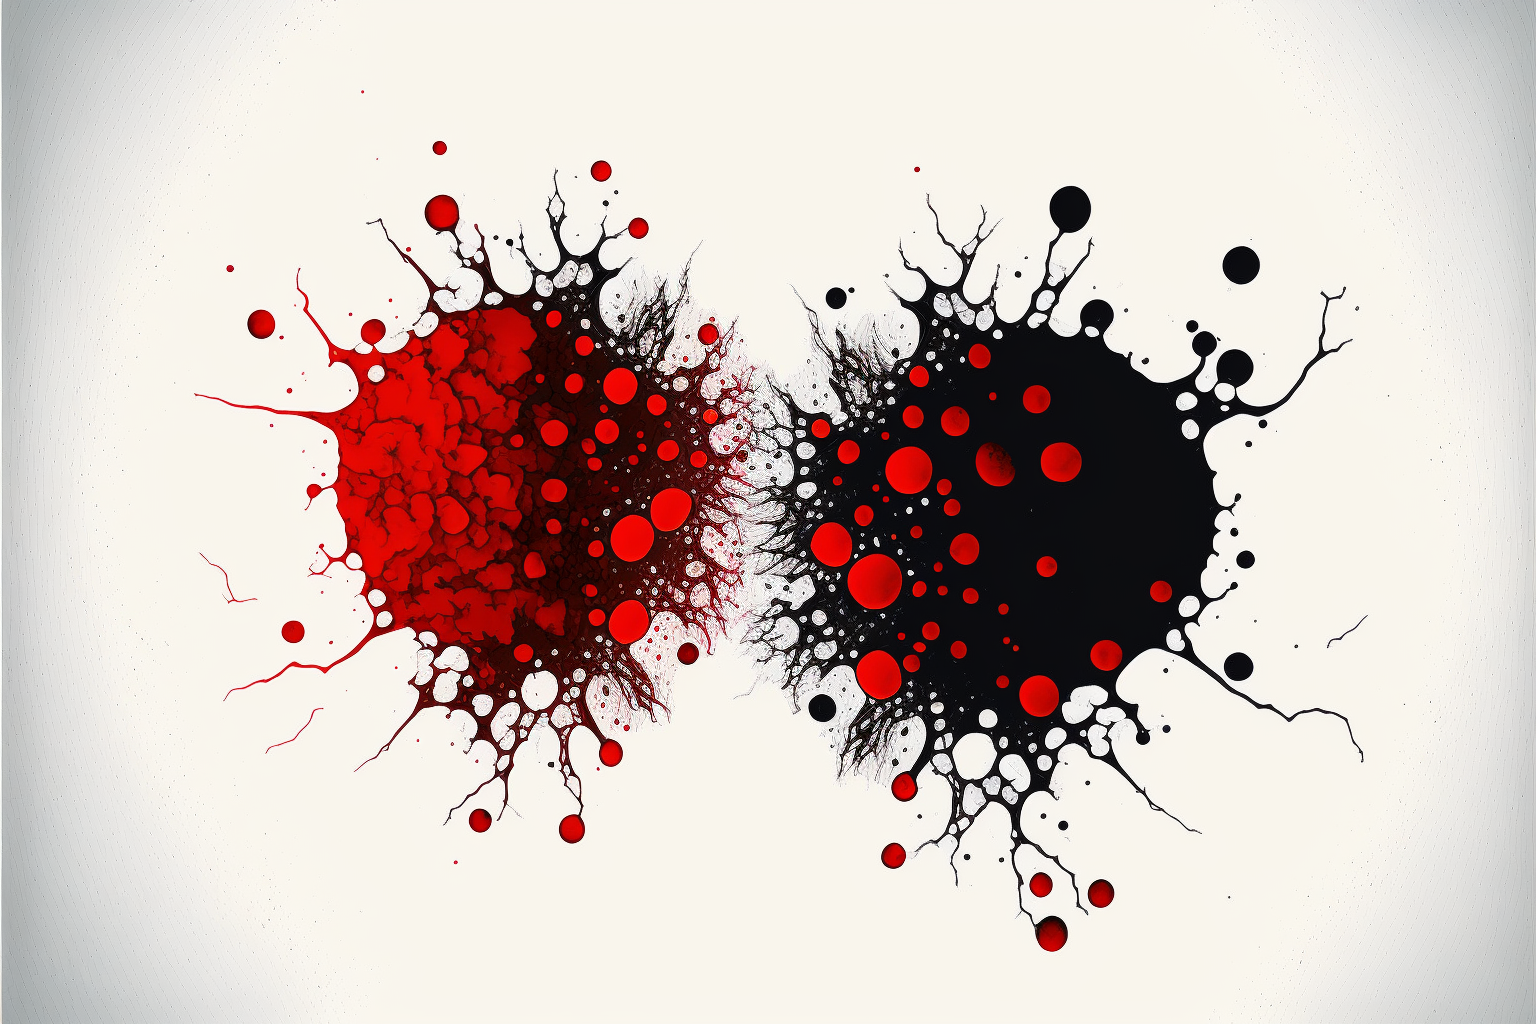
\includegraphics[height=10em]{chapters/ecpc.png}
% \end{figure}
% \vspace{-4cm}


\begin{changemargin}{0cm}{2cm}
\articletitle{Transcriptome analysis reveals an important role for pericytes in TNF-induced inflammatory response.}
\end{changemargin}

ALB Seynhaeve\textsuperscript{\ref{ecpc-affil:1}},
H Rasche\textsuperscript{\ref{ecpc-affil:3}},
Y Li\textsuperscript{\ref{ecpc-affil:3}},
WFJ van IJcken\textsuperscript{\ref{ecpc-affil:2}},
TLM ten Hagen\textsuperscript{\ref{ecpc-affil:1}}

\textbf{Manuscript In Preparation} \\

\small
\begin{enumerate}
\itemsep-0.5em

\item Laboratory of Experimental Oncology, Department of Pathology, Erasmus University Medical Center, 3015 GD Rotterdam, The Netherlands.\label{ecpc-affil:1}
\item  Center for Biomics, Erasmus University Medical Center, 3015 GD Rotterdam, The Netherlands.\label{ecpc-affil:2}
\item Clinical Bioinformatics, Department of Pathology, Erasmus University Medical Center, 3015 GD Rotterdam, The Netherlands.\label{ecpc-affil:3}
\end{enumerate}
\normalsize


\section*{Abstract}

TNF regulates the immune-response and is crucial in our defence against pathogens and is involved in wound healing, cardiac remodelling and cartilage regeneration. However, TNF is also involved in several inflammatory conditions such as rheumatoid arthritis, psoriasis, Crohn's disease, and sepsis and is linked to endothelial cell dysfunction and vascular leakage. Pericytes also play a role in vascular leakage and edema formation. Here we aim to better understand the role of pericytes in TNF-induced inflammation. For this we incubated pericytes and endothelial cells with medium and TNF, performed RNA sequencing and isolated the genes that were differential expressed in TNF-induced pericytes compared to naive pericytes and endothelial cells. Biologically TNF had no effect on pericyte and endothelial cell death and endothelial cell permeability despite a change in endothelial cell morphology. We found that genes of the inflammatory, IFN alpha and IFN gamma pathways were highly over-represented in TNF-induced pericytes compared to naïve and TNF-induced endothelial cells. Especially genes of the CXCL and CCL families were significantly upregulated.

To also understand the effect of these TNF-induced factors by pericytes on endothelial cells, we added TNF-conditioned pericyte medium on endothelial cells. We observed that factors produced by TNF-stimulated pericytes increased the endothelial cell permeability and morphology significantly and also further stimulated endothelial cells to express CXCL and CCL chemokines. This shows how endogenous produced factors between these two important cell types in the vasculature influence each other during TNF-induced inflammation.

\section*{Introduction}

Tumor necrosis factor alpha is an important inflammatory cytokine and plays an important role in our natural immunity to fight of infections and for tissue repair, cardiac remodeling and cartilage regeneration. However, TNF is also a key regulator of tissue degeneration and several autoimmune diseases. Blocking its action has been successful in treating and managing psoriasis, rheumatoid arthritis and inflammatory bowel disease although serious adverse effects of anti-TNF therapy have been reported ranging from severe bacterial infections, lupus-like reactions and even lymphoma development\cite{Bradley_2007,Tiegs_2022}. These opposite activities depend mainly on concentration, site of action, and presence of other factors. TNF is produced as a 26 kDa transmembrane precursor protein (mTNF) and is cleaved into a soluble 17 kDa protein (sTNF). Both proteins are biological active and trimerize upon binding to the receptor. There are two membrane receptors, P55 TNFR1 which is stimulated by mTNF as well as sTNF and P75 TNFR2 which is stimulated by mTNF. Activation of TNFR2 leads predominantly to inflammation, cell survival and cell proliferation and TNFR1, which contains a death domain, can also lead to cell death\cite{Tiegs_2022,Kalliolias_2015}. TNF regulates the immune-response and is therefore crucial in the defense against pathogens and is also involved in tissue repair, cardiac remodeling and cartilage regeneration. At higher doses, TNF is involved in apoptosis and cancer cell death. Additionally, TNF induces a shift to tissue degeneration and is involved in renal failure and neurological disorders such as Alzheimer disease and depression\cite{Miola_2021,How_Shing_Koy_2021}. Dysregulation of TNF is also involved in inflammatory diseases like rheumatoid arthritis, psoriasis, Crohn's disease, and sepsis\cite{Kalliolias_2015} and is linked to unwanted endothelial cell dysfunction and vascular leakage\cite{Ferrero_2001,Seynhaeve_2006,R_egg_1998}.

Cells of the vasculature, and especially endothelial cells, act as gatekeepers for fluid exchange and leucocytes transmigration during normal inflammation to destroy infiltrating pathogens, clear up destroyed tissue and start the repair process. Wound healing also involves angiogenesis, the growth of new vessels from existing ones, and is highly influenced by pro-inflammatory factors. Under normal circumstances tissue repair and angiogenesis are well regulated. However in pathological conditions, like chronic wound healing, asthma and cancer this balance is disturbed. It is still not exactly understood how local immune response contributes in a pro- or antiangiogenic behavior and more than likely there is a tipping point favoring the one above the other. This imbalance can result in autoimmune diseases in which the immune systems starts to attack its own body or, contradictory, in immune deficiency diseases preventing the immune system to respond to invaders. In tumors the balance is often in favor of tumor maintenance and growth as stromal cells such as endothelial cells, perivascular cells, fibroblasts and infiltrating immune cells creates a supporting framework and reservoir for local pro-tumoral and pro-angiogenic factors. Tumors are therefore often defined as wounds that never heals. We and others have shown previously that TNF can increase vascular leakage and permeability specifically in vascular region in which the vasculature is already compromised, like in a tumor\cite{Ferrero_2001,R_egg_1998,Seynhaeve_2006,8479472a627b42e19c2e2cf5c8505de7,Brouckaert_2004}.

Besides endothelial cells, perivascular cells (i.e. smooth muscle cells in larger vessels such as arteries and veins and pericytes in capillaries) are also a required cellular component to build a well conducting functional vascular network. These cells are considered the muscle of a vessel although their close molecular and biological connection with endothelial cells suggest they play a larger role than just support\cite{Seynhaeve_2018,Brandt_2019,Caporali_2017}. The participation of multiple cell types, producing several factors in a time- and dose dependent manner makes the relationship between immune response and angiogenesis a complex biological process to investigate.

To better understand the genetic involvement of pericytes in TNF-induced vascular permeability we compared the mRNA expression profile of TNF-stimulated pericytes compared to those of endothelial cells.

\section*{Materials And Methods}

\subsection*{Study design}

Endothelial cells and pericytes plated with a confluence of 80\% were incubated with medium or 1 µg/ml HuTNF for 12, 24 and 72 hours (\cref{figure:exp-design}). To extract RNA, TRIzol (Thermo Fisher Scientific) was added to the cells and collected. A total of 24 samples was collected with two samples per treatment and timepoint for each cell line. Secondly, endothelial cells were exposed, for 24 hours, to pericyte conditioned medium that have been cultured with medium or TNF (\cref{figure:exp-design}, right side) and 6 samples collected with 3 replicates per condition were collected: 3 for the control treatment, and 3 for the pericyte conditioned medium.

PureLink RNA Mini Kit (Thermo Fisher Scientific) was used for rapid purification of total RNA according to the manufacturer's instructions.

To obtain sufficient replicates for statistical power in the first dataset, we chose to collapse the time axis as it was not a strong contributor to variation. We analysed the principal components and conducted an ANOVA test on the count distributions for a selected panel of genes of interest to confirm the minimal effect of time on our samples. This resulted in 24 samples with 6 per condition set of conditions: cell type and presence or absence of TNF.to confirm the minimal effect of time on our samples. This resulted in 24 samples with 6 per condition set of conditions: cell type and presence or absence of TNF.

\begin{figure}[bt!]
\centering
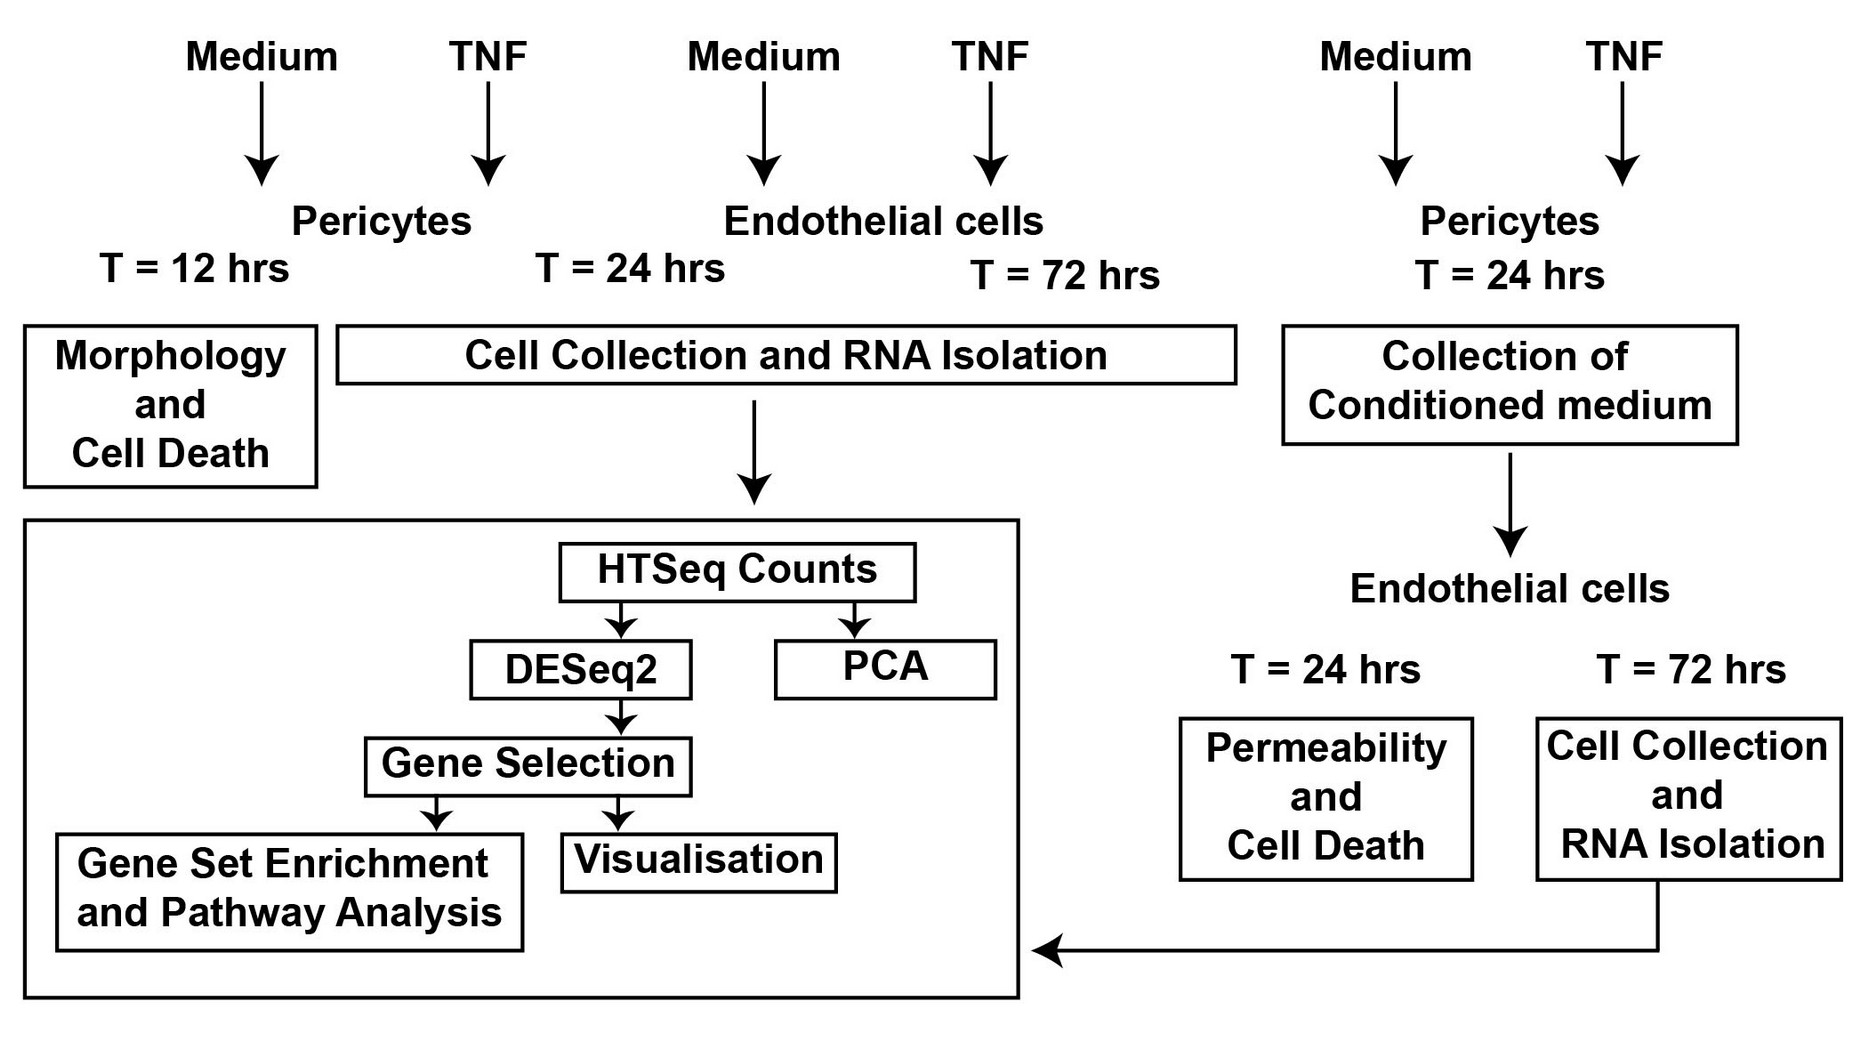
\includegraphics[width=\linewidth]{chapters/images/ecpc-000.png}
\caption{Schematic of the experimental design}\label{figure:exp-design}
\end{figure}

\subsection*{Cell culturing conditions}

Human umbilical vein endothelial cells (huvec) were isolated by collagenase digestion using the method described by Jaffe\cite{Jaffe_1973} and human pericytes from placenta were purchased from PromoCell GmbH. For maintenance and plating, cells were incubated in the most optimal cell culture medium. Endothelial cell medium contained human endothelial-serum free medium (Thermo Fisher Scientific), 20\% heat inactivated newborn calf serum (Thermo Fisher Scientific), 10\% heat inactivated human serum (Sigma-Aldrich), 20 ng/mL recombinant human basic Fibroblast Growth Factor (PeproTech EC Ltd), 100 ng/mL recombinant human Epidermal Growth Factor (PeproTech EC Ltd) and endothelial cells were plated on a gelatin (Sigma-Aldrich) coating\cite{Seynhaeve_2006} and pericytes were maintained in Pericyte Growth Medium 2 (PromoCell GmbH). To assess cell death, permeability and morphology changes cells were incubated with a 1/1 mixture huvec/pericyte medium and for RNA sequencing cells were incubated with DMEM/2\%FCS.

\subsection*{Cell dead, permeability and morphology assays}

To investigate direct effects of TNF, endothelial cells and pericytes cells plated with a confluence of 80\% were incubated with medium or 1 µg/ml HuTNF for 12, 24 and 72 hours (\cref{figure:exp-design}). Morphology of living cells was checked using a Zeiss 100M and thereafter fixed to analyse cell death using sulpharhodamin B (SRB, Sigma-Aldrich) as previously described\cite{Seynhaeve_2006}. Protein bound SRB was dissolved in 10 mM TRIS and optical density (OD) was measured at 540 nm. Cell growth was calculated using the formula: percentage cell growth = (O.D. test well/O.D. control well) x 100 percent.

For the preparation of conditioned medium (\cref{figure:exp-design}), pericytes plated in a 6 wells plate with a confluence of 80\% were incubated with medium or 1 µg/ml HuTNF for 24 hours. As a proper control a cell-free plate was handled the same way as the plate with pericytes. Medium was collected, centrifuged to remove cellular debris and stored at -20ºC until further use. Permeability of the endothelial cell monolayer and measuring length-to-width ratio was performed as previously described\cite{Seynhaeve_2006,Seynhaeve_2014}. Briefly, endothelial cells were plated in the upper chamber of a transwell (0.4 µm pore size, Corning) and allowed to reach confluence. Medium in the upper chamber was replaced with conditioned medium and FITC-BSA. After the incubation time, FITC fluorescence in the lower chamber was measured using a fluorescence plate reader (Wallac Victor2, PerkinElmer). Endothelial cells were imaged with a 10x N.A. 0.30 Plan-Neofluar objective lens using an inverted Zeiss Axiovert 100M microscope equipped with an Axiocam digital camera (Carl Zeiss). Cell elongation was measured and expressed as the ratio of the length of the major cell axis to the width perpendicular to the length.

\subsection*{Cell collection for RNA sequencing}

\subsection*{RNA sequencing}

RNA-Seq library was prepared for analysis according to the Illumina TruSeq stranded mRNA protocol as previously described\cite{Birkhoff_2020,Heshusius_2022}. Briefly, poly containing mRNA from 200 ng of total RNA using poly-T oligos attached magnetic beads. The poly-A mRNA was fragmented, and cDNA was synthesized using SuperScript II and random primers in the presence of Actinomycin D. cDNA fragments were end repaired, purified with AMPure XP beads, A-tailed using Klenow exo-enzyme in the presence of dATP. Paired-end adapters with dual index were ligated to the A-tailed cDNA fragments and purified using AMPure XP beads. The resulting adapter-modified cDNA fragments were enriched by PCR using Phusion polymerase as followed: 30 s at 98°C, 15 cycles of 10 s at 98°C, 30 s at 60°C, 30 s at 72°C, and ending with 5 min at 72°C. PCR products were purified using AMPure XP beads and eluted in 30 µl of resuspension buffer. One microliter was loaded on an Agilent Technologies 2100 Bioanalyzer using a DNA 1000 assay to determine concentration and quality check. Cluster generation was performed according to the Illumina TruSeq SR Rapid Cluster kit v2 Reagents Preparation Guide. Briefly, for sequencing libraries were pooled together to get a stock of 10 nM and one microliter of this stock was denatured with NaOH, diluted to 10 pM and hybridized onto the flow cell. The hybridized products were sequentially amplified, linearized and end-blocked according to the Illumina Single Read Multiplex Sequencing user guide. After hybridization of the sequencing primer, sequencing-by-synthesis was performed on a HiSeq 2500 instrument. Single reads were generated of 50 base-pairs in length. These were mapped to the human reference genome version GRCh38 using HISAT2\cite{Kim_2015}. Gene expression counts for the CCDS genes were calculated using HTseq-count\cite{Anders_2014} and the Ensembl release 96 transcript annotation\cite{Howe_2020}.

\section*{Data analysis}

In the first experiment the data analysis sought to identify expression changes in genes and pathways in both endothelial cells and pericyte separately, through differential gene expression analysis. In the second we explored the effect of pericyte conditioned medium to explore its effects on gene expression in endothelial cells. For both experiments, first the variance of the underlying data was explored, differential expression tested, and differential expression of pathways analysed.

\begin{figure}[bt!]
\centering
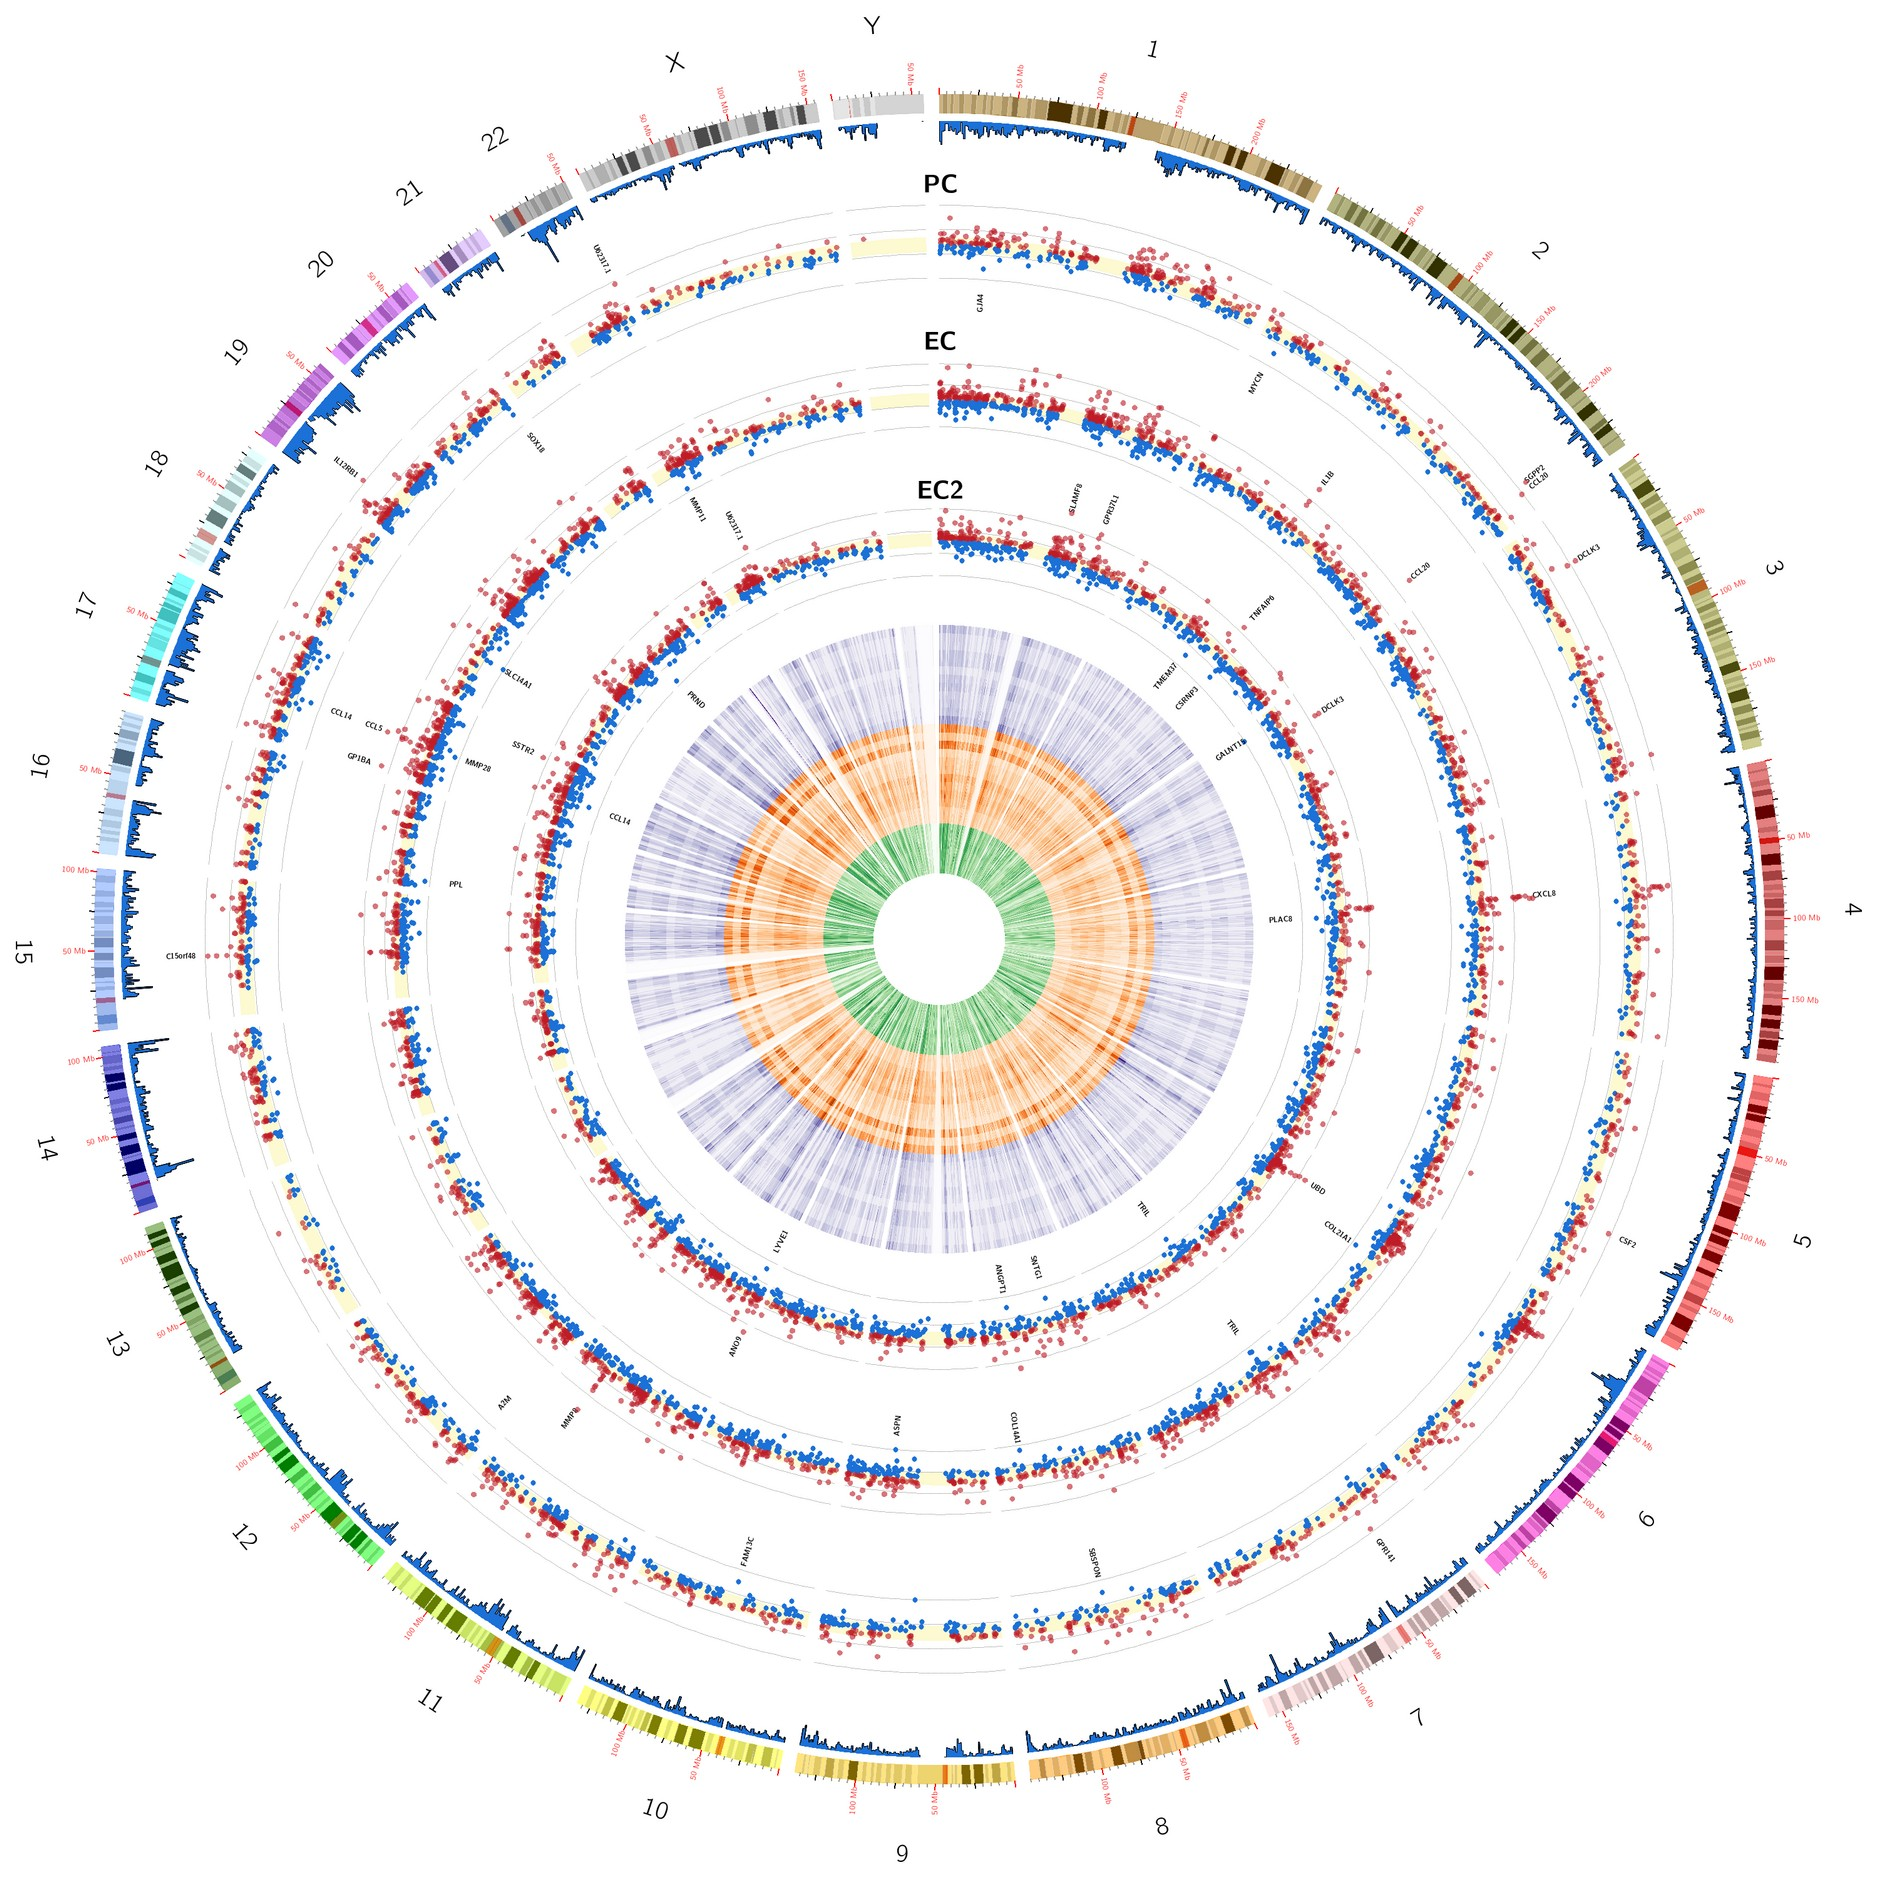
\includegraphics[width=\linewidth]{chapters/images/ecpc-001.png}
\caption{Differential expression from the two experiments, producing three compraisons is shown here. A number of chemokines are seen upregulated. In the centre the RNA sequencing coverage is plotted, indicating similar overall expression patterns between samples, while showing some banding due to the experimental conditions.}\label{figure:circos}
\end{figure}

In comparing the responses of endothelial cells and pericytes to TNF (\cref{figure:exp-design}), to identify the large sources of variance, the HTseq-count files were analysed with the variance stabilising transform (VST) via DESeq2 in R to produce a Principal Component Analysis (PCA) plot.

As we were primarily interested in the gene expression changes due to TNF treatment, we chose a simple model for analysing the results of the first experiment which only looked at the changes due to TNF treatment, in both Endothelial and Pericyte cells separately. This was repeated for the second experiment as well, comparing only TNF vs the control condition.

Differential gene expression was performed using DESeq2\cite{Love_2014} (\cref{figure:exp-design}) which models expression using the negative binomial distribution. The analysis was conducted using the default p-value adjustment of Benjamini-Hochberg. The first experiment provided 6 replicates per condition sets, with conditions of cell type (endothelial, pericyte) and treatment (TNF, ctrl). The cell types were expression tested separately with DESeq2 with the only condition being their treatment, as the expression changes due to cell type were an unnecessary source of variance in the analysis, in a group of 6 replicates per condition (TNF, ctrl). Resulting expression changes for both cell types were filtered based on the cutoff criteria of an adjusted p-value \textless{} 0.05.

Gene set enrichment analysis was performed with the ReactomePA for each resulting set of differentially expressed genes (adj. p-val \textless{} 0.05). All pathways available in Reactome were included in the analysis, and the resulting p-values adjusted with Benjamini-Hochberg. Results were filtered for adj. P-val \textless{} 0.05.

\section*{Results}

\subsection*{Cell death and morphology changes}

Pericytes and endothelial cells were exposed to medium and TNF for 12, 24 and 72 hours. Morphology, cell dead and genetic expression was analyzed. Adding TNF on pericytes and endothelial cells had no effect on cell death (\cref{figure:cells}). TNF had no effect on pericyte morphology and induced cell elongation in endothelial cells correlation with previous findings\cite{Seynhaeve_2006}.

\begin{figure}[bt!]
\centering
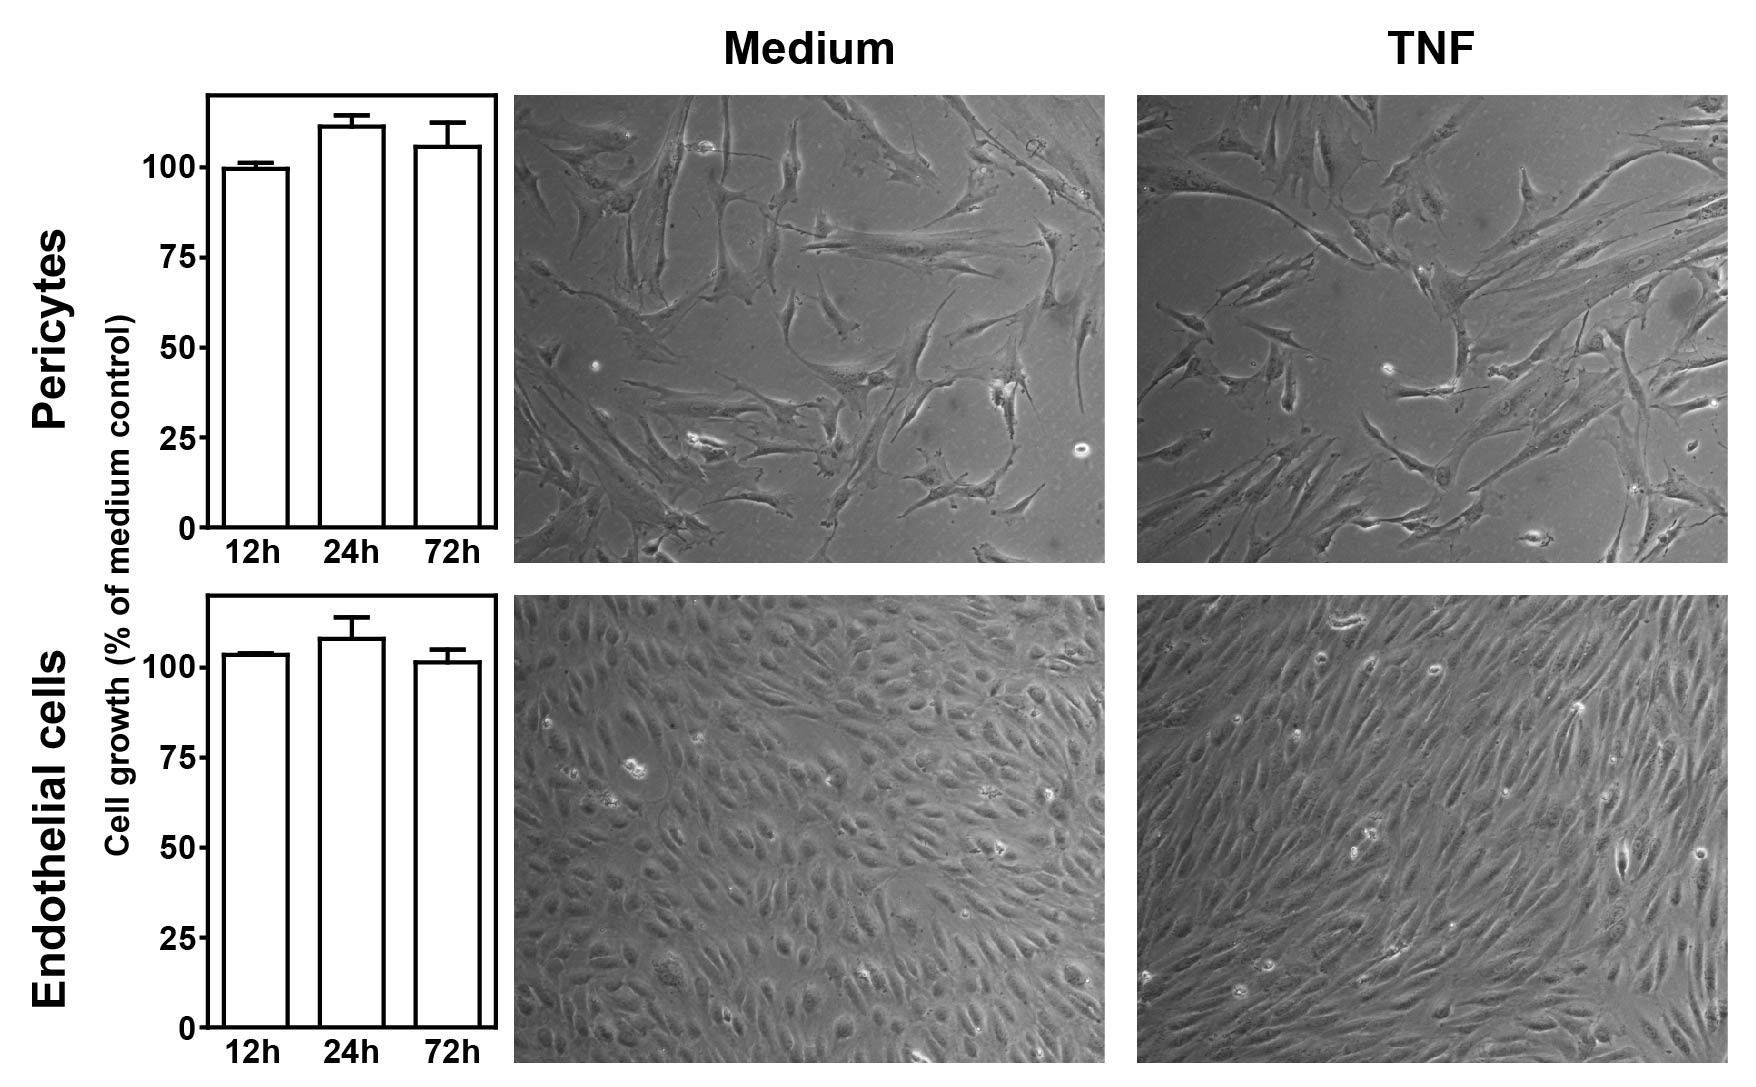
\includegraphics[width=\linewidth]{chapters/images/ecpc-003.png}
\caption{Cell growth and morphological changes of pericytes and endothelial cells. Shown is that TNF has no effect on cell death and minimal effect on cell morphology as TNF induces some elongation in endothelial cells.}\label{figure:cells}
\end{figure}

% Fig 3. Cell growth and morphological changes of pericytes and endothelial cells. Shown is that TNF has no effect on cell death and minimal effect on cell morphology as TNF induces some elongation in endothelial cells.

\subsection*{Source of Variance}

Examining the PCA plot of the HTSeq counts, 80\% of the variance is explained by celltype, 13\% by treatment with some potential minor variation in Endothelial cells due to time (\cref{figure:pca1}).

\begin{figure}[bt!]
\centering
\includegraphics[width=\linewidth]{chapters/images/ecpc/4-pca.png}
\caption{Principal Component Analysis (PCA) of sequencing data obtained from the first experiment, indicating strong separation based on cell type and secondarily on treatment condition.}\label{figure:pca1}
\end{figure}
% Fig 4. 

These principal components influenced our decision to collapse the time axis in order to have a sufficient number of replicates. We further confirmed that time was not a major factor with a qualitative examination of a pre-selected panel of genes of interest (chemokines involved in inflammatory pathways: \emph{TNF, CXCL1, CXCL8, CX3CL1, IL1, IL17, IFNA1}) via examination of their VST-adjusted counts, which showed strong trends for genes of interest for factors of cell type and treatment condition, with no observable strong relationship for time (\cref{figure:sup1}). An ANOVA analysis identified condition (F=553.8) as the primary factor, next to celltype (F=7.227) and time (F=2.199) for \emph{TNF}.

\subsection*{TNF-induced transcriptional changes}

Under the comparison of interest (TNF vs control), across both pericytes and endothelial cells we observed a total of 1674 genes were differentially expressed in this experiment (adjusted p-value \textless{} 0.05, abs(Log\textsubscript{2}(FoldChange)) ≥ 1.5).

\begin{figure}[bt!]
\centering
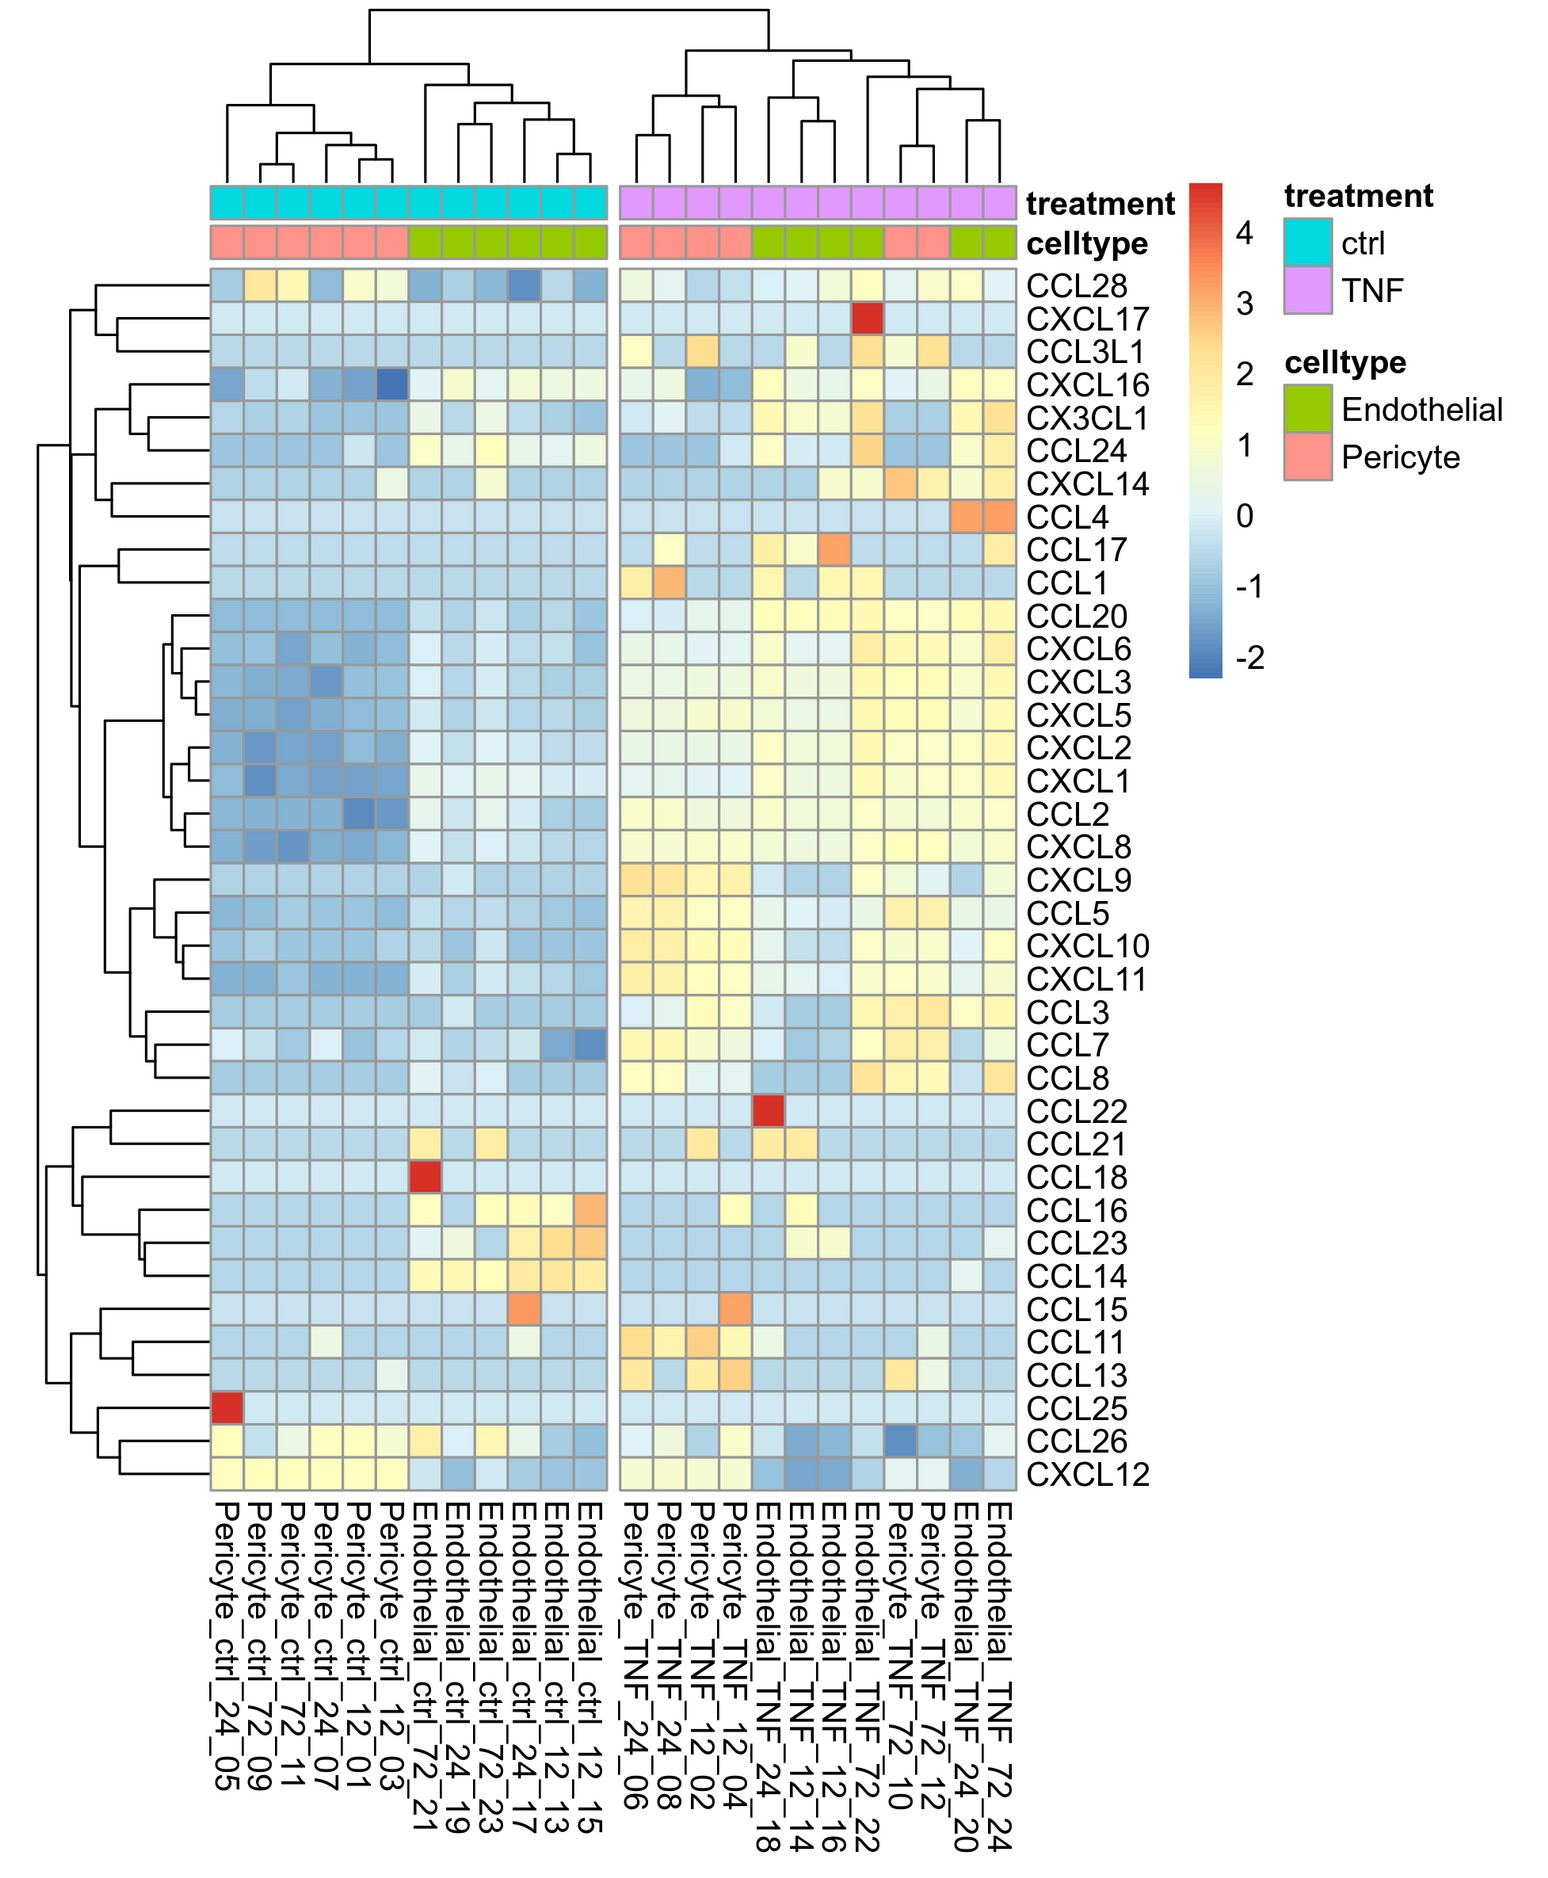
\includegraphics[width=\linewidth]{chapters/images/ecpc-006.png}
\caption{Heatmap of z-scores across CXCL and CCL genes. In contrast to the PCA analysis, expression patterns cluster strongly around treatment followed by cell type, for CXLC and CCL cytokines.}\label{figure:heatmap}
\end{figure}

Of these 1057 were differentially expressed in pericytes and 617 in endothelial cells. This is approximately 7.3\% of protein coding features present in Ensembl release 96 indicating that TNF is a significant gene expression modulator.

\begin{figure}[bt!]
\centering
\includegraphics[width=\linewidth]{chapters/images/ecpc/deg_upset.png}
\caption{Pericytes experience the strongest change with many uniquely up and down regulated genes, Endothelial Cells showing about half as many uniquely differentially expressed genes. Nevertheless there are a significant number of genes which are either up-, or down-regulated in both cell types.}\label{figure:ggupset}
\end{figure}

The most strongly upregulated genes are all characterised by being chemokines or related in some way to inflammation (\cref{table:genesendo,table:genesperi}). Notably CXCL6 which regulates cell permeability%
% https://pubmed.ncbi.nlm.nih.gov/33241954/{]}
is overexpressed in both cell types.

\begin{table}[h!t]
    \footnotesize
    \label{table:genesendo}
	\centering
	\begin{tabular}{|ll|ll|}
		\hline
		Gene ID & Gene Name & log2FoldChange &Adjusted P-Value \\ \hline

		\hline
		ENSG00000163082 & SGPP2    & 10.13 & 2.40E-19 \\
		ENSG00000163673 & DCLK3    & 9.40  & 1.55E-08 \\
		ENSG00000096996 & IL12RB1  & 8.65  & 9.76E-06 \\
		ENSG00000115009 & CCL20    & 7.92  & 1.54E-116 \\
		ENSG00000166920 & C15orf48 & 7.63  & 1.13E-10 \\
		ENSG00000164400 & CSF2     & 7.58  & 2.78E-21 \\
		ENSG00000187037 & GPR141   & 7.44  & 1.87E-06 \\
		ENSG00000124875 & CXCL6    & 7.40  & 2.86E-10 \\
		ENSG00000108342 & CSF3     & 7.12  & 1.98E-10 \\
		ENSG00000140522 & RLBP1    & 6.75  & 2.91E-07 \\
		ENSG00000174640 & SLCO2A1  & -3.68 & 2.73E-12 \\
		ENSG00000073737 & DHRS9    & -3.78 & 3.80E-12 \\
		ENSG00000255690 & TRIL     & -3.83 & 6.08E-07 \\
		ENSG00000203883 & SOX18    & -3.89 & 2.41E-40 \\
		ENSG00000175899 & A2M      & -3.90 & 3.02E-13 \\
		ENSG00000134323 & MYCN     & -4.16 & 6.42E-07 \\
		ENSG00000148541 & FAM13C   & -4.36 & 1.46E-04 \\
		ENSG00000164764 & SBSPON   & -4.37 & 2.96E-04 \\
		ENSG00000187513 & GJA4     & -4.68 & 1.16E-03 \\
		ENSG00000276409 & CCL14    & -4.81 & 3.28E-06 \\\hline
	\end{tabular}
    \caption{Top 10 Up- and Down-regulated genes in Endothelial cells exposed to TNF vs control}
\end{table}

\begin{table}[h!t]
    \footnotesize
    \label{table:genesperi}
	\centering
	\begin{tabular}{|ll|ll|}
		\hline
		Gene ID & Gene Name & log2FoldChange &Adjusted P-Value \\ \hline

		\hline
		ENSG00000169245 & CXCL10  & 13.14 & 3.53E-24 \\
		ENSG00000118113 & MMP8    & 12.78 & 1.14E-12 \\
		ENSG00000169248 & CXCL11  & 12.34 & 2.12E-24 \\
		ENSG00000115009 & CCL20   & 12.32 & 1.25E-10 \\
		ENSG00000271503 & CCL5    & 11.77 & 1.20E-86 \\
		ENSG00000125538 & IL1B    & 11.67 & 2.34E-174 \\
		ENSG00000169429 & CXCL8   & 11.38 & 2.95E-164 \\
		ENSG00000185245 & GP1BA   & 10.54 & 5.12E-18 \\
		ENSG00000179826 & MRGPRX3 & 10.08 & 2.37E-17 \\
		ENSG00000124875 & CXCL6   & 10.07 & 4.19E-17 \\
		ENSG00000117115 & PADI2   & -4.77 & 1.26E-05 \\
		ENSG00000255690 & TRIL    & -5.16 & 2.02E-05 \\
		ENSG00000118898 & PPL     & -5.37 & 1.07E-07 \\
		ENSG00000241644 & INMT    & -5.37 & 6.94E-16 \\
		ENSG00000187955 & COL14A1 & -5.39 & 1.85E-07 \\
		ENSG00000271447 & MMP28   & -5.39 & 1.12E-03 \\
		ENSG00000124749 & COL21A1 & -5.53 & 1.02E-14 \\
		ENSG00000099953 & MMP11   & -5.64 & 9.38E-12 \\
		ENSG00000141469 & SLC14A1 & -6.50 & 5.54E-09 \\
		ENSG00000106819 & ASPN    & -6.53 & 1.35E-06 \\\hline
	\end{tabular}
    \caption{Top 10 Up- and Down-regulated genes in Pericytes exposed to TNF vs control}
\end{table}

\subsection*{TNF stimulated expression of CXCL and CCL chemokines in pericytes}

Among these pathways a predominant role was found of CXCL and CCL chemokines. CXCL1, 2, 3, 5, 6, 8, 10, and 11 were all found to be overexpressed in \emph{both} endothelial cells and pericytes when compared to their respective controls, however in all cases a stronger overexpression was observed in pericytes than endothelial cells; on the order of \textasciitilde32-64 times more strongly in pericytes relative to endothelial cells, across each measured gene, whilst endothelial cells themselves were over expressed on the order of 32 times versus their control. CXCL9 overexpression was only observed in pericytes.

A similar observation can be made for the CCL family of chemokines, CCL 2,3,5,7,8,13,11 and 20 are all significantly and strongly upregulated in Pericytes. Many of these are likewise significantly overexpressed, though endothelial cells are not as consistently upregulated as they are for CXCLs.

\begin{figure}[bt!]
\centering
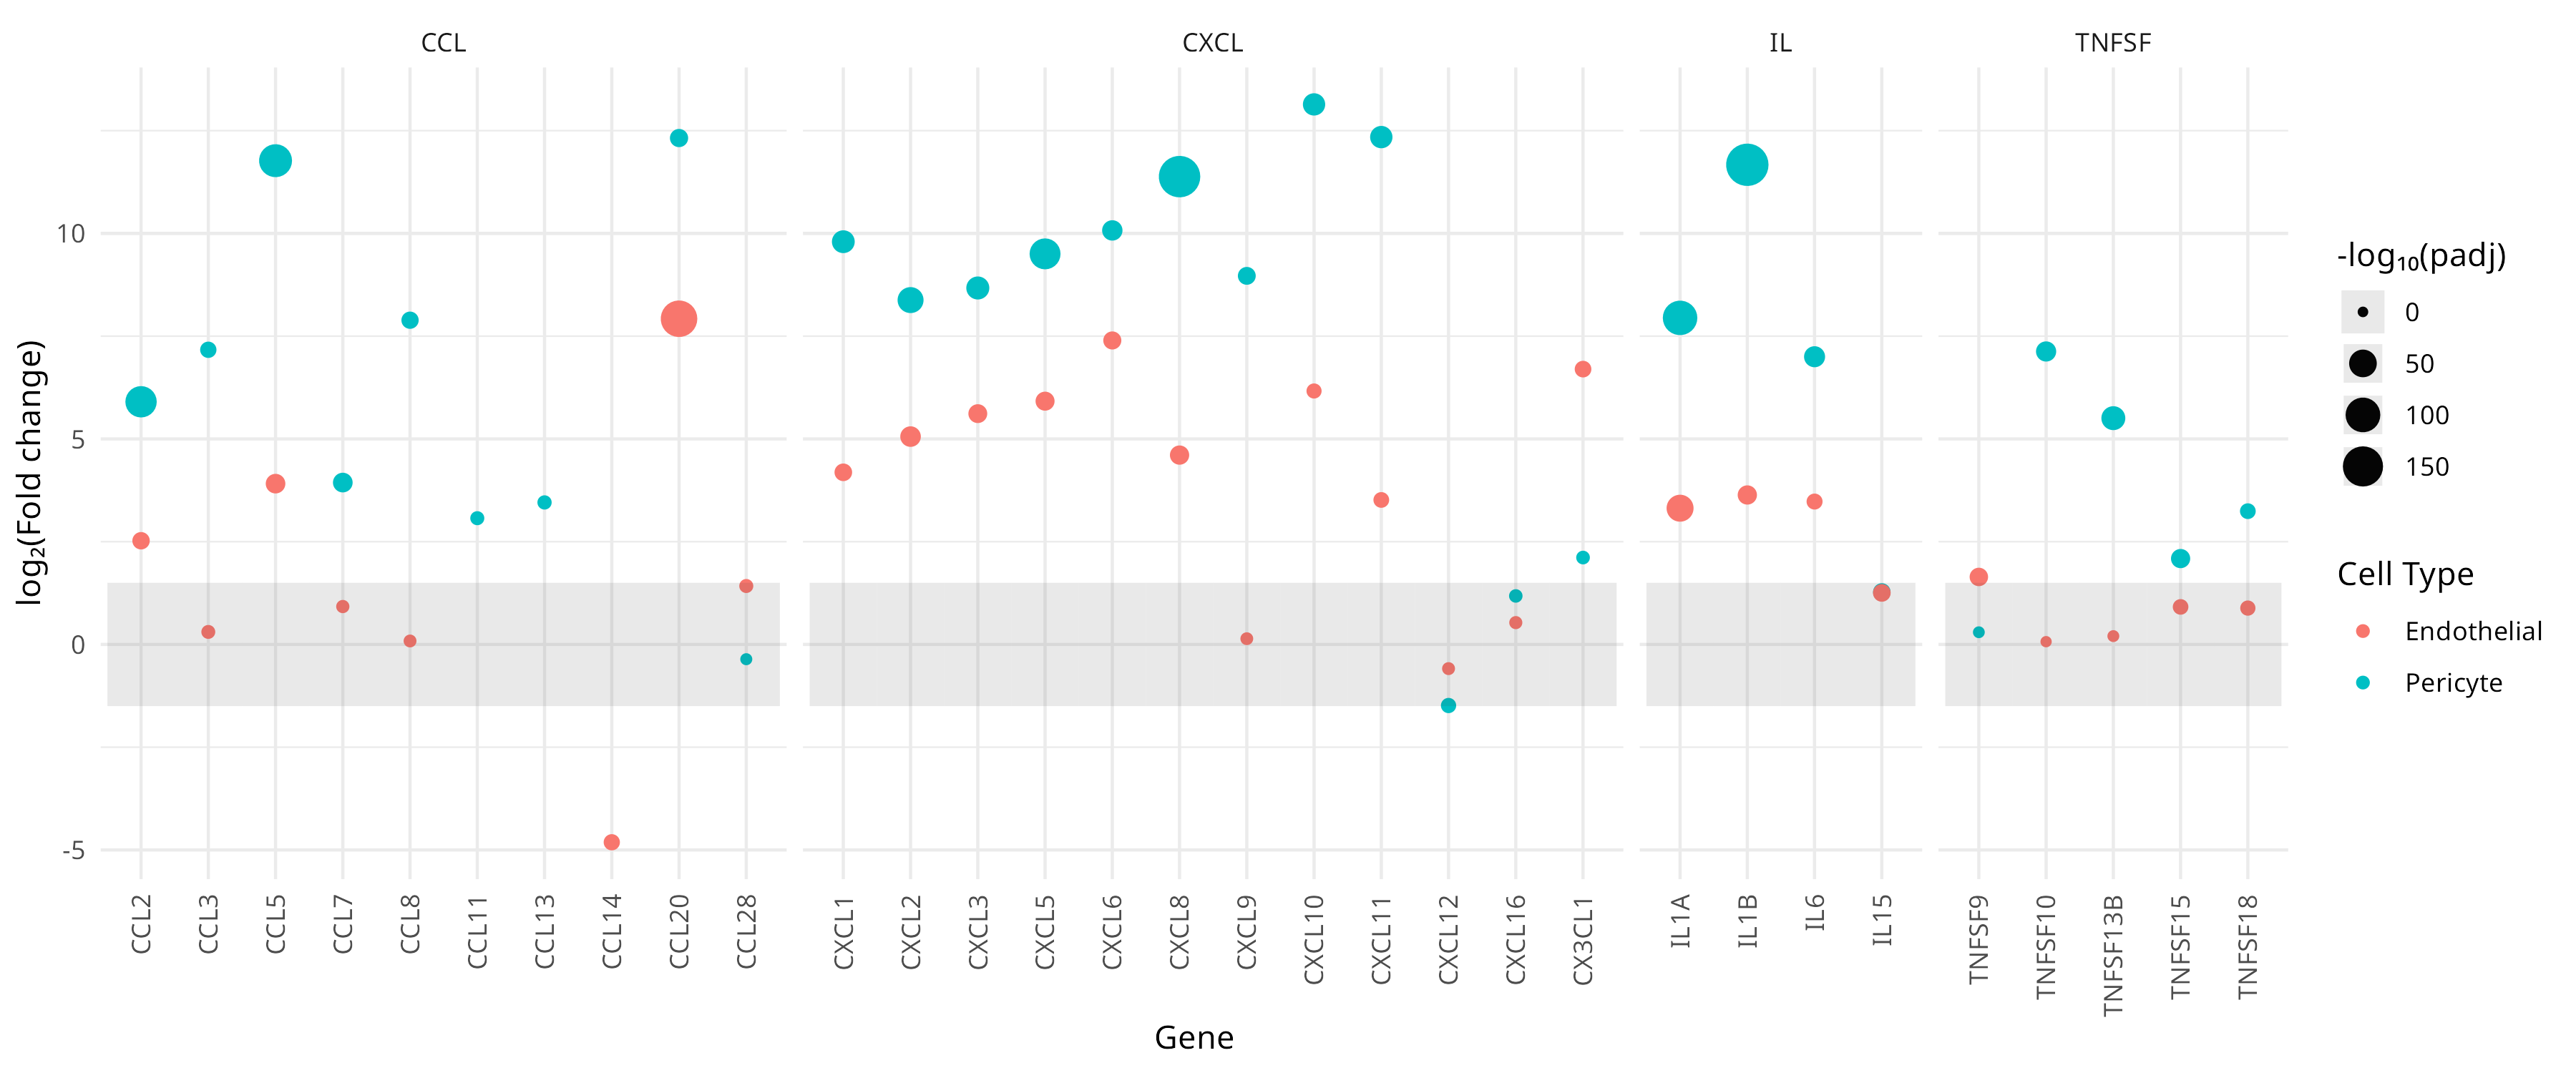
\includegraphics[width=\linewidth]{chapters/images/ecpc/chemokines-4.png}
\caption{Fold change upregulation of CXCL family chemokines in both Pericytes and Endothelial cells when exposed to TNF versus control treated pericytes and endothelial cells. In most cases TNF is responsible for a 32-64 times higher upregulation in pericytes compared to endothelial cells. The grey stripe indicates the region where the absolute Log₂ Fold Change is \textless1.5. Upregulation of CCL chemokines follows a similar pattern as CXCL. Interleukins produce a similar response pattern, however the upregulation is less pronounced in ECs. TNF Super Family proteins only show significant (padj\textless0.05, abs(L2FC)≥1.5) primarily in Pericytes.}\label{figure:foldchange}
\end{figure}

To better understand the genes that were differentially expressed, we conducted gene set enrichment analysis using the significantly using the Reactome database via ReactomePA%
%{[}CITATION GOES HERE,\href{https://doi.org/10.1039/C5MB00663E}{doi:10.1039/C5MB00663E}{]}
. 90 pathways were over-expressed; 10 only in Endothelial cells under TNF, 37 only in Pericytes, and 43 observed in both. Overall, pathways related to immunological responses dominated the genes overexpressed in TNF-stimulated pericytes and endothelial cells. The cytokine-signalling, interleukin signalling, and immune pathways showed the strongest up-regulation (\cref{table:pathways}).

% \emph{Table 3: }

\begin{table}[h!t]
    \footnotesize
    \label{table:pathways}
	\centering
	\begin{tabular}{llll}
		\hline
		\multicolumn{3}{c}{\textbf{Endothelial}}\\\hline
		ID            & Description                          & Adjusted P-Value \\\hline
		R-HSA-168256  & Immune System                        & 2.52E-27 \\
		R-HSA-1280215 & Cytokine Signaling in Immune system  & 3.97E-23 \\
		R-HSA-449147  & Signaling by Interleukins            & 1.24E-13 \\
		R-HSA-375276  & Peptide ligand-binding receptors     & 2.77E-11 \\
		R-HSA-6783783 & Interleukin-10 signaling             & 2.43E-09 \\
		R-HSA-373076  & Class A/1 (Rhodopsin-like receptors) & 1.25E-08 \\
		R-HSA-380108  & Chemokine receptors bind chemokines  & 1.29E-08 \\
		R-HSA-168249  & Innate Immune System                 & 1.11E-07 \\
		R-HSA-913531  & Interferon Signaling                 & 3.04E-07 \\
		R-HSA-500792  & GPCR ligand binding                  & 8.15E-07 \\\hline
		\multicolumn{3}{c}{\textbf{Pericytes}} \\\hline
		ID            & Description                          & Adjusted P-Value \\\hline
		R-HSA-1280215 & Cytokine Signaling in Immune system  & 1.69E-34 \\
		R-HSA-449147  & Signaling by Interleukins            & 5.54E-17 \\
		R-HSA-6783783 & Interleukin-10 signaling             & 7.88E-15 \\
		R-HSA-913531  & Interferon Signaling                 & 2.96E-14 \\
		R-HSA-375276  & Peptide ligand-binding receptors     & 1.30E-12 \\
		R-HSA-909733  & Interferon alpha/beta signaling      & 9.53E-11 \\
		R-HSA-380108  & Chemokine receptors bind chemokines  & 9.53E-11 \\
		R-HSA-373076  & Class A/1 (Rhodopsin-like receptors) & 2.48E-10 \\
		R-HSA-168249  & Innate Immune System                 & 1.61E-08 \\
		R-HSA-418594  & G alpha (i) signalling events        & 4.38E-08 \\\hline
	\end{tabular}
    \caption{Top 10 most significantly over-represented pathways due to differentially expressed genes in TNF treated ECs and PCs relative to their controls. Pathway enrichment was accomplished via ReactomePA with a p-value threshold of 0.05.}
\end{table}

\subsection*{Pericytes involvement in TNF-induced endothelial permeability}

Non cell- and pericyte-conditioned medium was made by adding medium or TNF to an empty well or wells with pericytes and incubate for 24 hours, there after conditioned medium was collected and added to endothelial cells for 72 hours to check morphology and permeability changes and 24 hours to preform RNA sequencing as described above. We measured that pericytes medium conditioned with TNF increased permeability in the endothelial monolayer significantly compared to the other conditions (\cref{table:lwr}). TNF changed endothelial cell morphology from a coble stone monolayer to a more elongated shape represented as length-to-width ration (1.65 ± 0.07 vs 4.86 ± 0.53) and this was even more pronounced when combined with pericytes medium conditioned with TNF (7.99 ± 0.04) (\cref{table:lwr,figure:cells2}). This indicates that a TNF-induced endogenous factors produced by pericytes are of high influence in the permeability of an endothelial monolayer.

\begin{figure}[bt!]
\centering
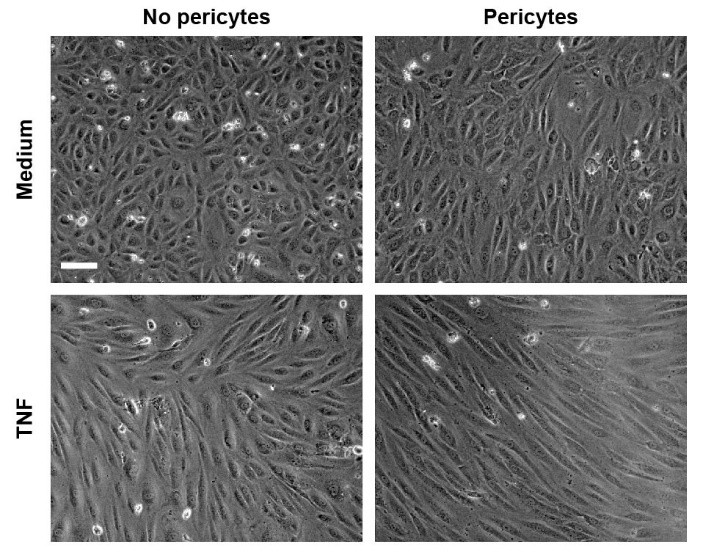
\includegraphics[width=\linewidth]{chapters/images/ecpc-011.png}
\caption{Changes in endothelial cells morphology when cells were exposed to conditioned medium from pericytes. Shown is that conditioned medium from TNF-stimulated pericytes induces morphological changes in the endothelial layer.}\label{figure:cells2}
\end{figure}

\begin{table}[h!t]
    \footnotesize
	\centering
	\begin{tabular}{l|ll|ll}
		\hline
		Conditioned Medium    & \multicolumn{2}{c}{No Cells}                            & \multicolumn{2}{c}{PC}\\
		TNF                   & No                           & Yes                      & No             & Yes \\\hline
		Permeability          & 104.7 ± 3.6*                 & 110.2 ± 1.5*             & 115.3 ± 9.9*   & 164.4 ± 10.9 \\
		Length-to-width ratio & 1.65 ± 0.07*\#\$             & 4.86 ± 0.53*             & 2.22 ± 0.15*\# & 7.99 ± 0.04 \\\hline
	\end{tabular}
	\caption{Endothelial cell permeability and length-to width ratio after incubation with conditioned medium. Endothelial cells were incubated with no cells-conditioned medium +/- TNF or pericyte-condition medium +/- TNF for 72 hours and permeability was analysed as \% of medium control and length-to-width ratio calculated. Data represent average ± SEM of 3 independent experiments. *, P \textless{} 0.05 versus PC + TNF; \#, P \textless{} 0.05 versus No cells + TNF; \$, P \textless{} 0.05 versus PC + No TNF}\label{table:lwr}
\end{table}

\subsection*{Higher expression of CXCL and CCL chemokine in endothelial cells exposed to TNF-conditioned pericyte medium.}

In the second experiment, we added incubated Pericytes with TNF before exposing Endothelial cells to that conditioned medium (TNF-PCCM) and performed RNA sequencing on the treated samples and a control. Samples were again decomposed with PCA showing that the replicates are very comparable (\cref{figure:sup2}). Differential expression analysis with DESeq2 identified 783 differentially expressed genes (adjusted p-value \textless{} 0.05, abs(log\textsubscript{2}FC)\textgreater1.5), 372 down-regulated and 411 up-regulated in endothelial cells that were incubated with medium versus TNF-conditioned pericyte medium (\cref{figure:ggupset}).

A similar pattern of upregulation is seen in endothelial cells when exposed to the TNF-conditioned pericyte medium. The pattern of expression changes in CCL genes match those of the first condition, when endothelial cells were exposed directly to TNF (\cref{figure:foldchange3}).

In comparison to TNF treated ECs, TNF-PCCM treated ECs respond very similarly, albeit with fewer significantly differentially expressed genes (783 vs 1383)

\begin{figure}[bt!]
\centering
\includegraphics[width=\linewidth]{chapters/images/ecpc/chemokines-7.png}
\caption{CXCL, CCL, IL, and TNSF genes exhibit similar regulation patterns to their TNF exposed counterparts.}\label{figure:foldchange2}
\end{figure}

\begin{figure}[bt!]
\centering
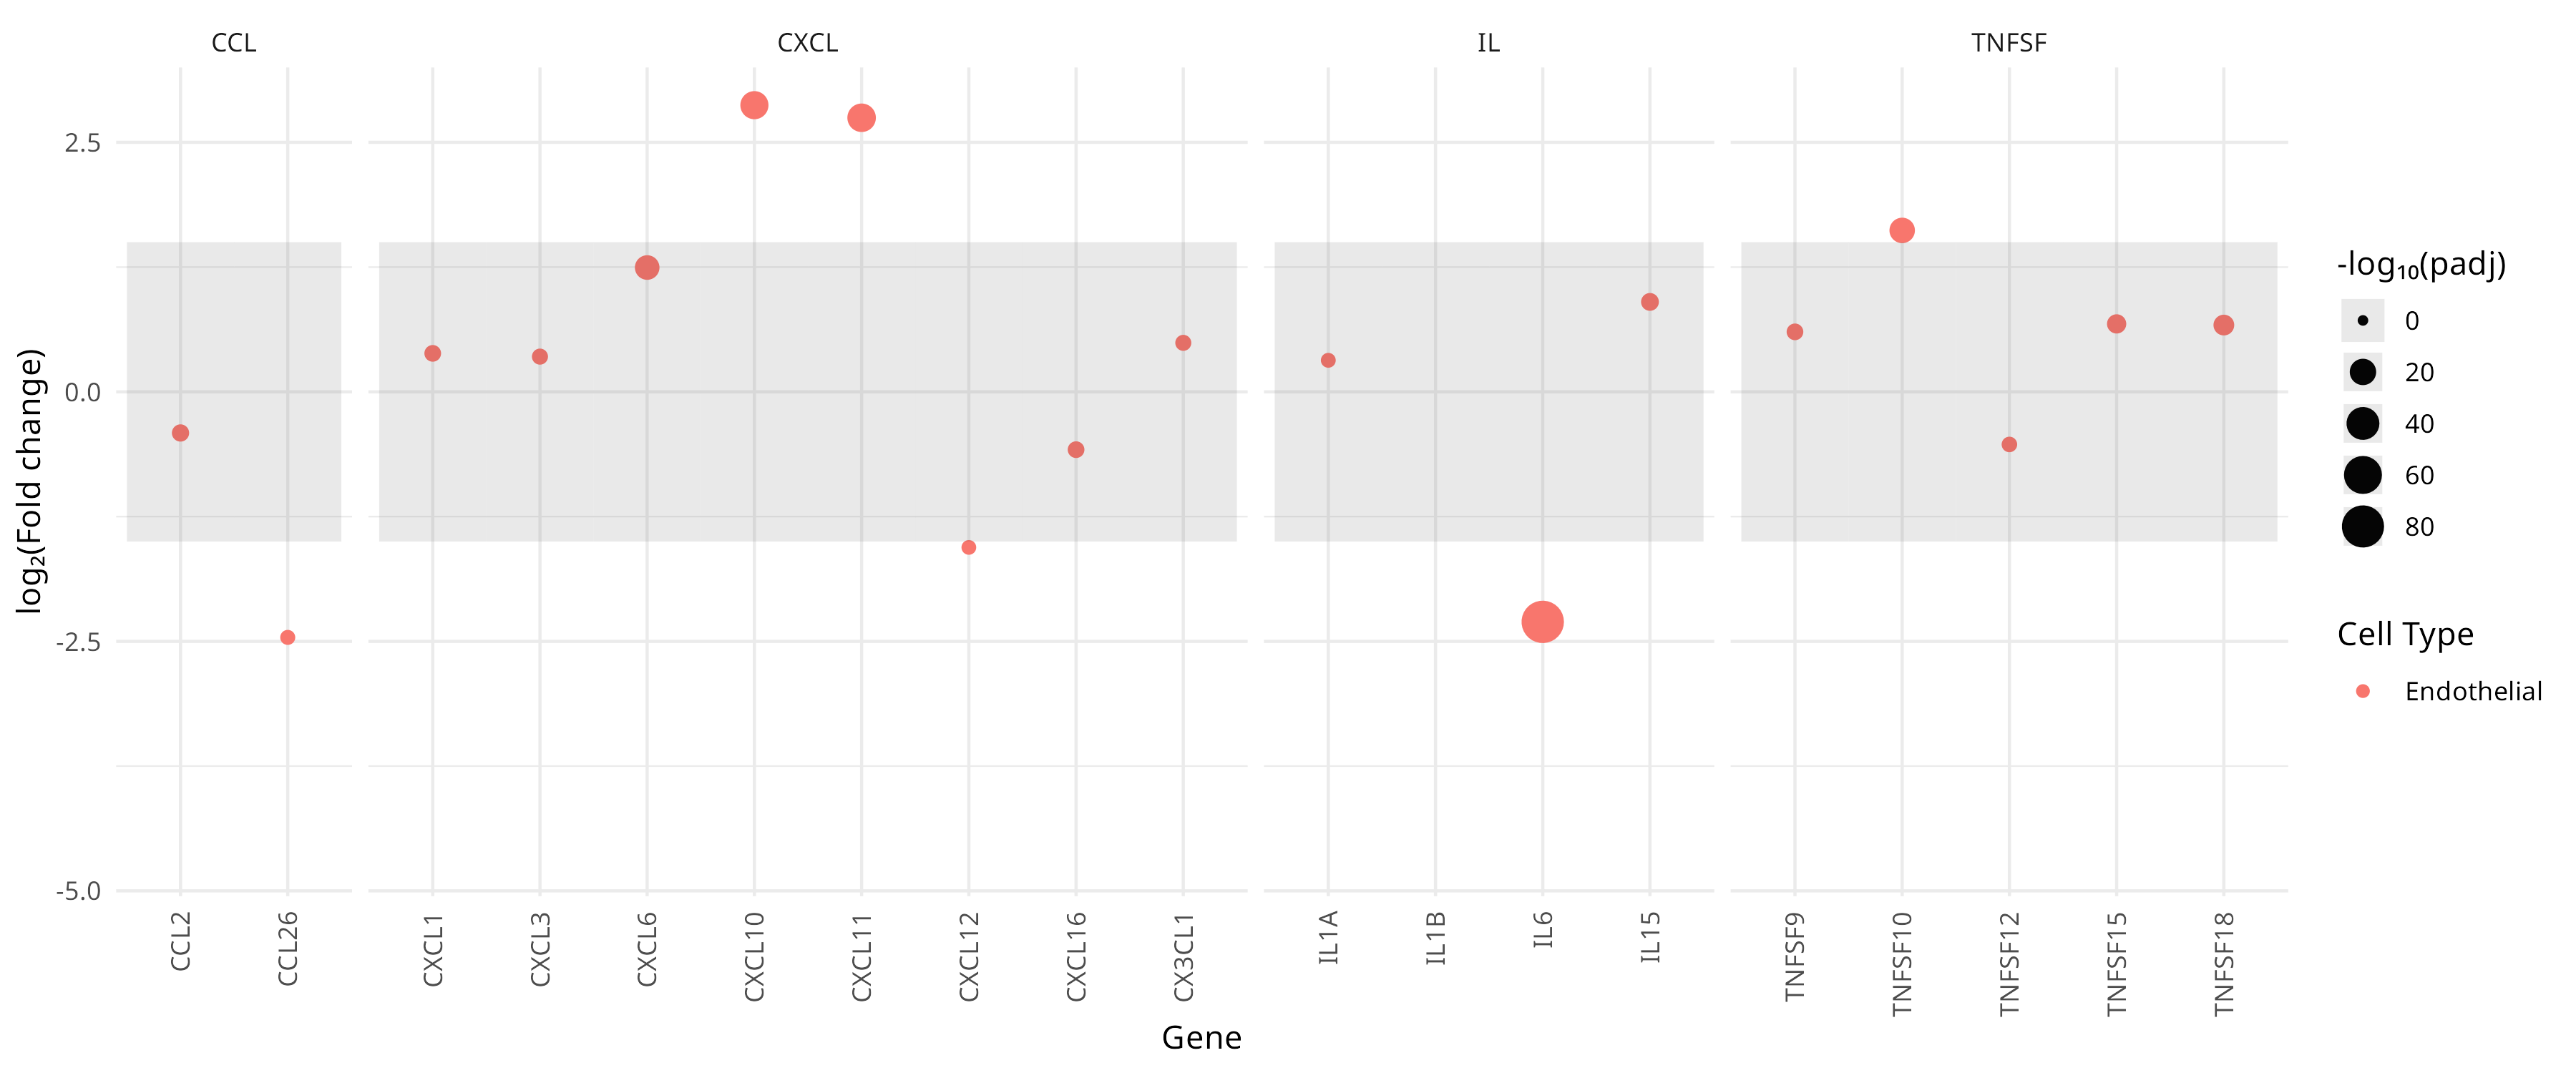
\includegraphics[width=\linewidth]{chapters/images/ecpc/chemokines-4v7.png}
\caption{Direct comparison of TNF-PCCM treated ECs versus TNF exposed ECs shows a much weaker trend, with upregulation of CXCL10 and CXCL11, and mild downregulation of IL6. However, in all cases, these genes were upregulated when compared to their controls.}\label{figure:foldchange3}
\end{figure}

\section*{Discussion}

Endothelial cells exist in close proximity with pericytes and this interaction defines the physicals properties and functions of specific blood vessels. We have recently shown the dynamic interaction between endothelial cells and pericyte in tumor angiogenesis and pericyte importance in maintenance of a functional blood flow\cite{Seynhaeve_2018,Seynhaeve_2021}. Pericytes have been implicated in a wide range of roles including stabilization and contractility of the vasculature, survival of endothelial cells, regulating vascular permeability and controlling immune cell homeostasis\cite{T_r_k_2021,Kaushik_2021}. Because of the morphological diversity, organ-specific characteristics, lack of common markers and unknown origins, pericytes and smooth muscle cells are difficult to identify\cite{Muhl_2020} and challenging to investigate. The most known and studied interaction is between endothelial cells, pericytes and astrocytes of the blood brain barrier\cite{Netzahualcoyotzi_2024}. Pericytes are crucial to regulate blood flow in response to neural activity or vasoactive agents for normal brain function. Also brain pericytes produce pleiotrophin, a neurotropic growth factor and lack of this growth factor leaves neuron susceptible to ischemic injury\cite{Nikolakopoulou_2019}. Degeneration of pericytes leads to immune cell infiltration to the brain responsible for neurological disorders as Alzheimer's and Parkinson's disease. As pericytes play such an important role in the growth and maintenance of a functional vasculature, these cells also gained more interest as a therapeutic target for tumor treatment over recent years. However, it is still inconclusive whether targeting pericytes is beneficial for tumor therapy as there are reports showing that patients with a higher PDGFR-alpha and -beta pericyte coverage have a better higher overall and progression free survival in metastatic colorectal cancer\cite{Mezheyeuski_2016} and Cooke et al showed that targeting pericytes can promote metastasis\cite{Cooke_2012}.

The effect of TNF, an important player in multiple immunological diseases involving disruption of the structural integrity of the vasculature, is mainly focused on immune cells and endothelial cells. Also, we have previously reported the importance of TNF towards endothelial cells dead, morphology and permeability changes in the concept of tumor vessel manipulation for cancer treatment \cite{Seynhaeve_2007,hoving2005addition}. However these effects were not a direct results of TNF but rather a result of interleukin-1 beta produced via TNF-stimulated peripheral blood mononuclear cells\cite{Seynhaeve_2006}. Also the presence of interferon-gamma was a requirement for integrity changes of the endothelial cell layer\cite{Seynhaeve_2006,R_egg_1998}. However, as pericytes are essential for the maintenance of vascular integrity we wanted to investigate the effects of TNF on these cells and especially the endogenous factors that are produced and the additional effect of these factors on endothelial cells. Here, we report that TNF directly has minimal physical effect on endothelial cells and pericytes, however an indirect effect in which endogenous produced factors by TNF stimulated pericytes damaged the endothelial cell integrity is seen by endothelial cell morphology changes and an increased permeability. Pericytes have been identify as producers of a wide range of pro-inflammatory cytokines and chemokines after stimulation\cite{Kaushik_2021,Guijarro_Mu_oz_2014} and comparing endothelial cells with pericytes our RNA sequencing data shows that pathways of the immune response are highly enriched in TNF exposed pericytes compared to non-exposed and TNF exposed endothelial cells. Especially the chemokines are expressed significantly higher in pericytes after TNF exposure compared to endothelial cells.

Chemokines are small secreted proteins that have essential roles in the immune response as the primary function is to regulate the interaction between immune cells and recruit these immune cells into tissue\cite{Hughes_2018}. Many of these chemokines are highly inducible in response to inflammatory stimuli and are even stimulated by other chemokines and play a role in most inflammatory diseases and, because of the continuous immunological stimuli in the tumor microenvironment, have also become an important therapeutic target for cancer treatment\cite{Li_2022}. Immune cell infiltration into the underlying tissue means transmigration though the vascular wall which includes endothelial cells and pericytes. Using confocal imaging Girbl et al nicely demonstrated the TNF-induced luminal trans-endothelial cell migration and the subluminal crawling of neutrophils in the space between endothelial cells and pericytes which was mediated by endothelial produced CXCL1 and neutrophil produced CXCL2\cite{Girbl_2018,Li_2022}. However, many processes are already in motion before transmigration occurs as primary location of inflammation are often within the tissue and pericytes are targeted before endothelial cells. Moreover, next to higher cytokine expression in TNF-stimulated pericytes, factors produced by pericytes even further stimulating chemokine production by endothelial cells. This was especially the case for CXCL10 which is significantly higher expressed in TNF-stimulated pericytes and also in endothelial cells stimulated with pericytes produced endogenous factors creating a feed back loop. Various chemokines including CCL2, CCL4 and CXCL-10 are involved in SARS-CoV-2 mediated infection attracting immune cells to the site of infection, further releasing additional cytokines also creating a pro-inflammatory feedback loop damaging the blood brain barrier and lungs\cite{Jakhmola_2020,Khalil_2021}. CXCL10 has recently been identified as a strong biomarker for patient outcomes in COVID-19\cite{Lor__2021}.

Pericytes also obtained a more dominant role in the tumor microenvironment via communication with endothelial cells, immune- and tumor cells and targeting these pericytes could improve cancer treatment strategies. As wounds that never heals, the tumor microenvironment is rich in stimulatory cyto- and chemokines. Moreover, tumor cells overexpress proteins that prevent destruction by the T-cells and even have the ability to adapt their own microenvironment in such a manner that growth is stimulated\cite{Wargo_2016}. In the past we have used TNF to specifically target the tumor-associated vasculature and subtle permeability changes in this tumor-associated vasculature increased co-administered chemotherapy concentration in the tumor resulting in an increased tumor effect\cite{Seynhaeve_2007}. While we focus in this report between the expression difference between TNF-stimulated endothelial cells and pericytes we have strong indications that pericytes play an important role in TNF-induced drug delivery.

\subsection*{Future work}

Further work should be done to investigate the dose response, and interactions between pericytes and endothelial cells, and identify factors affecting expression behaviour and communication patterns between PCs and ECs. Additionally obtaining further replicates at additional timepoints alongside imaging, in order to eliminate time-based variability would let us better understand the relationships between expression and cellular changes over time. Important data that is missing in this paper is the translation of the genomics data to protein production, using proteomics, luminex or ELISA assays as production of cytokines and binding to their respective receptors is the pathway to initiate biological and physcial effects in the immune response.

\section*{Conclusion}

TNF stimulated endothelial cells and pericytes both showed significant increases in expression of CXCL and CCL family cytokines, both natively in the presence of TNF, and in the presence of TNF-conditioned pericyte medium.

\section*{Data Availability}

Sequencing data is available on SRA (ID TBA). The R script and associated Conda environment for reproducibility are available on \href{https://github.com/ErasmusMC-Bioinformatics/ecpc}{GitHub} (Zenodo: doi:TBA).

\section*{Supplementary Data}

\begin{figure}[bt!]
\centering
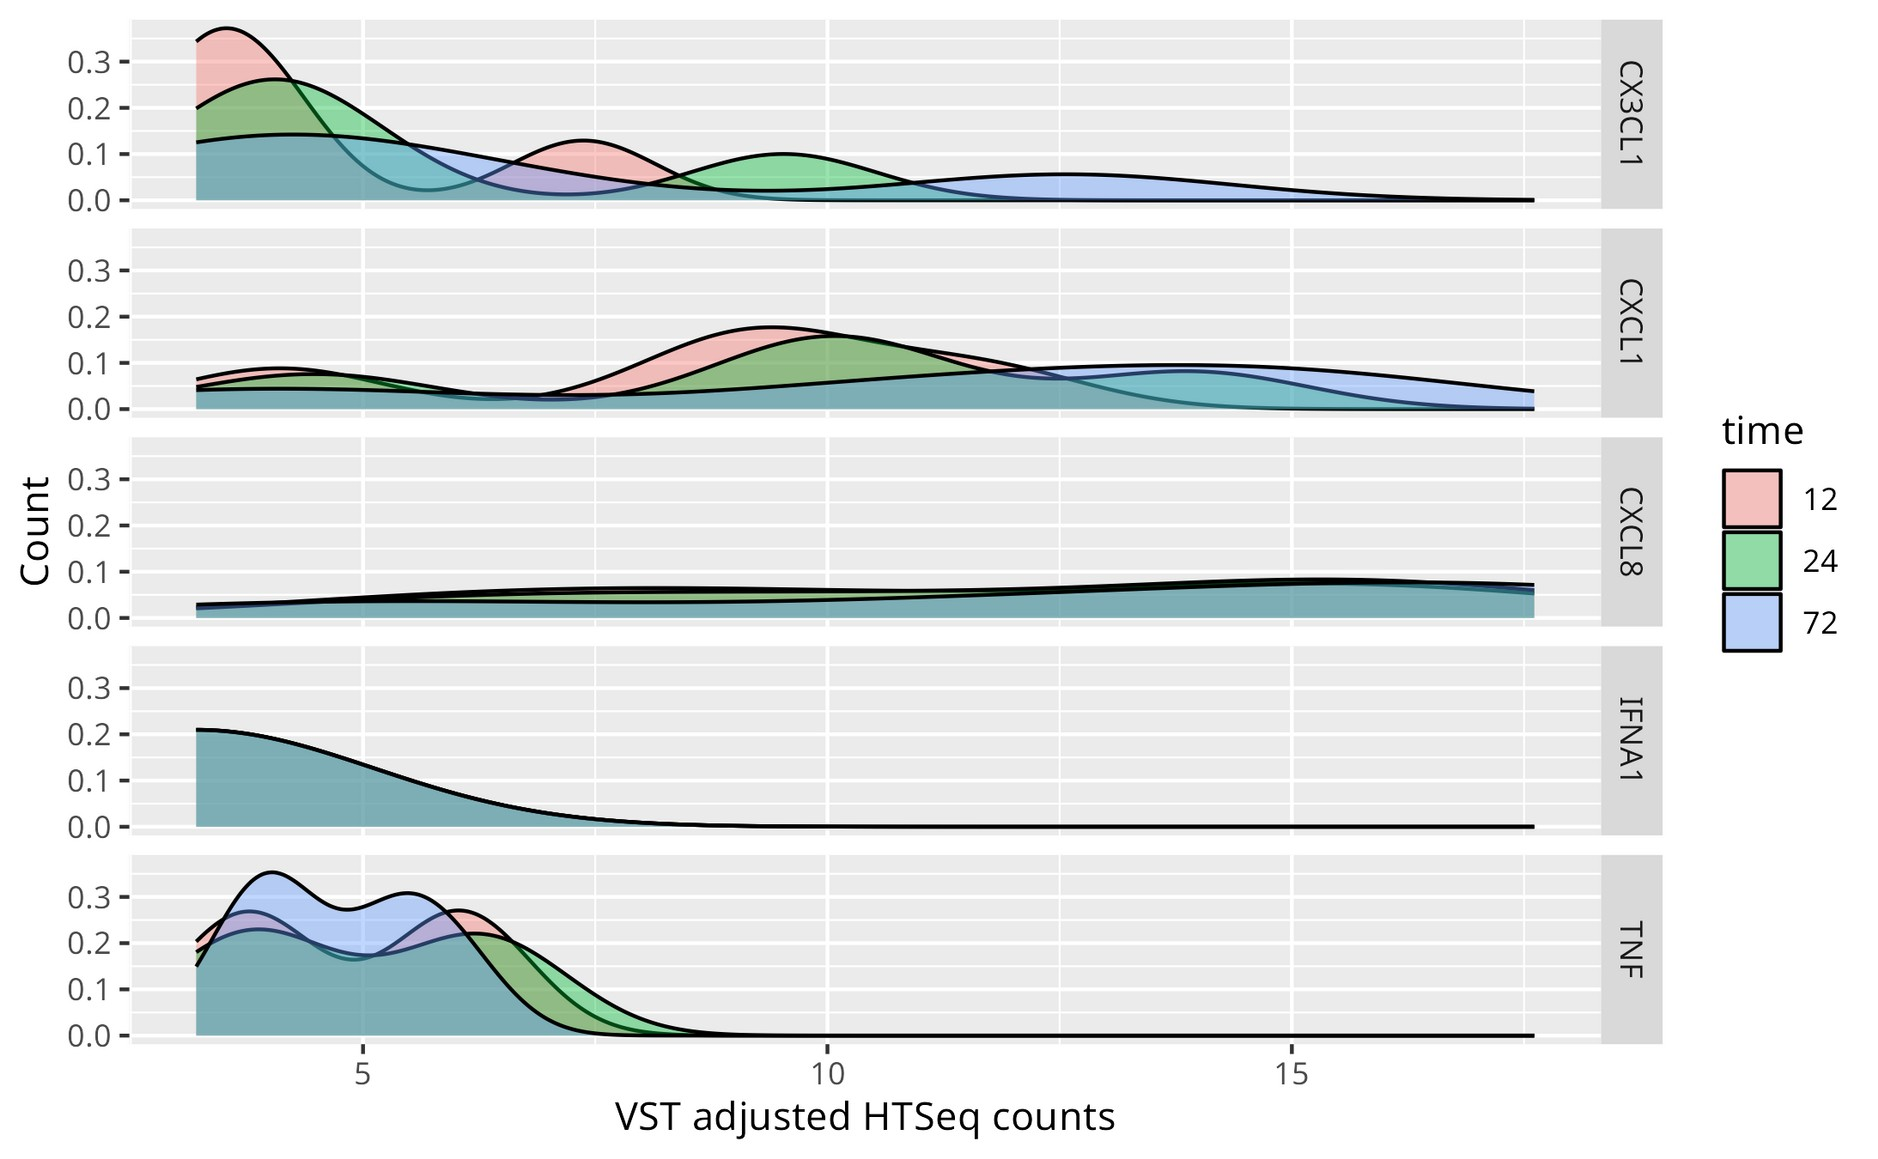
\includegraphics[width=0.7\linewidth]{chapters/images/ecpc-016.png}
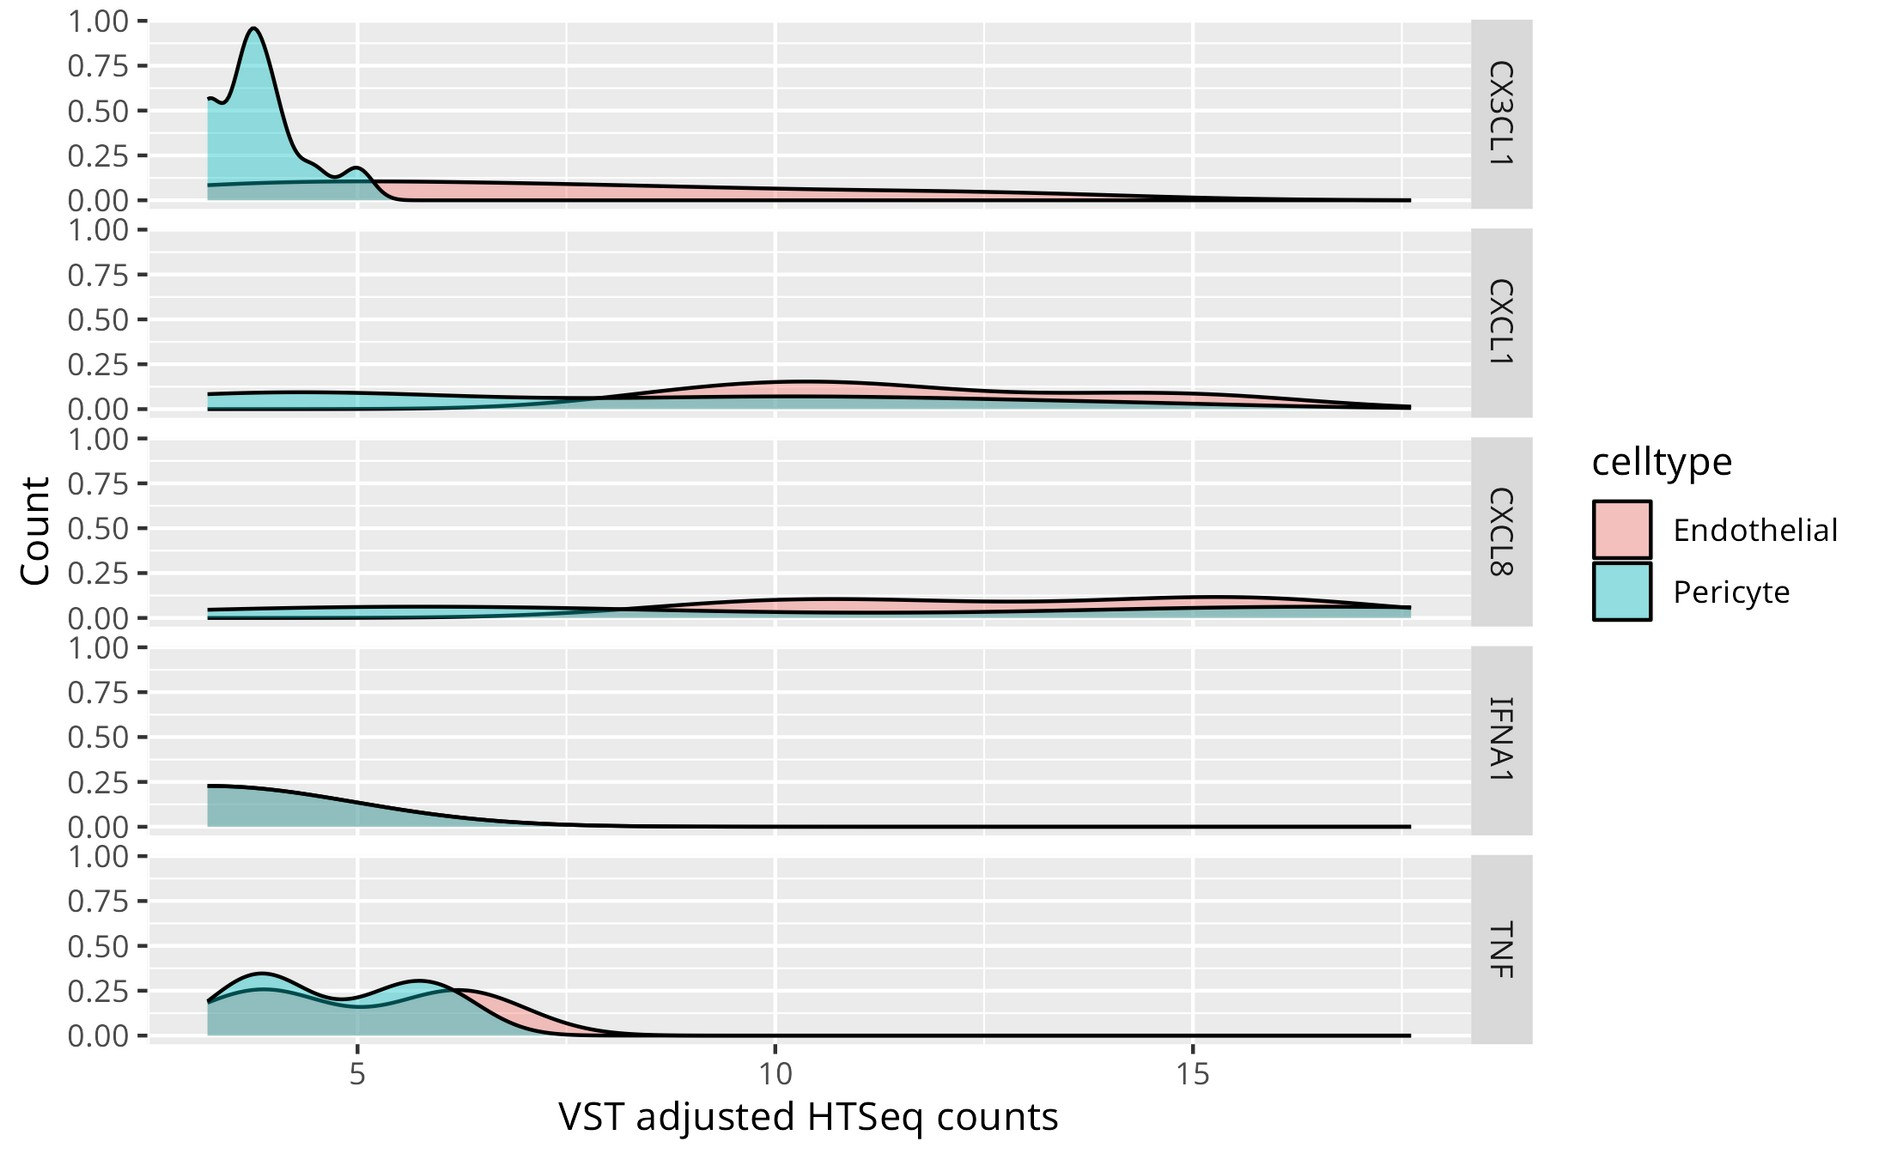
\includegraphics[width=0.7\linewidth]{chapters/images/ecpc-017.png}
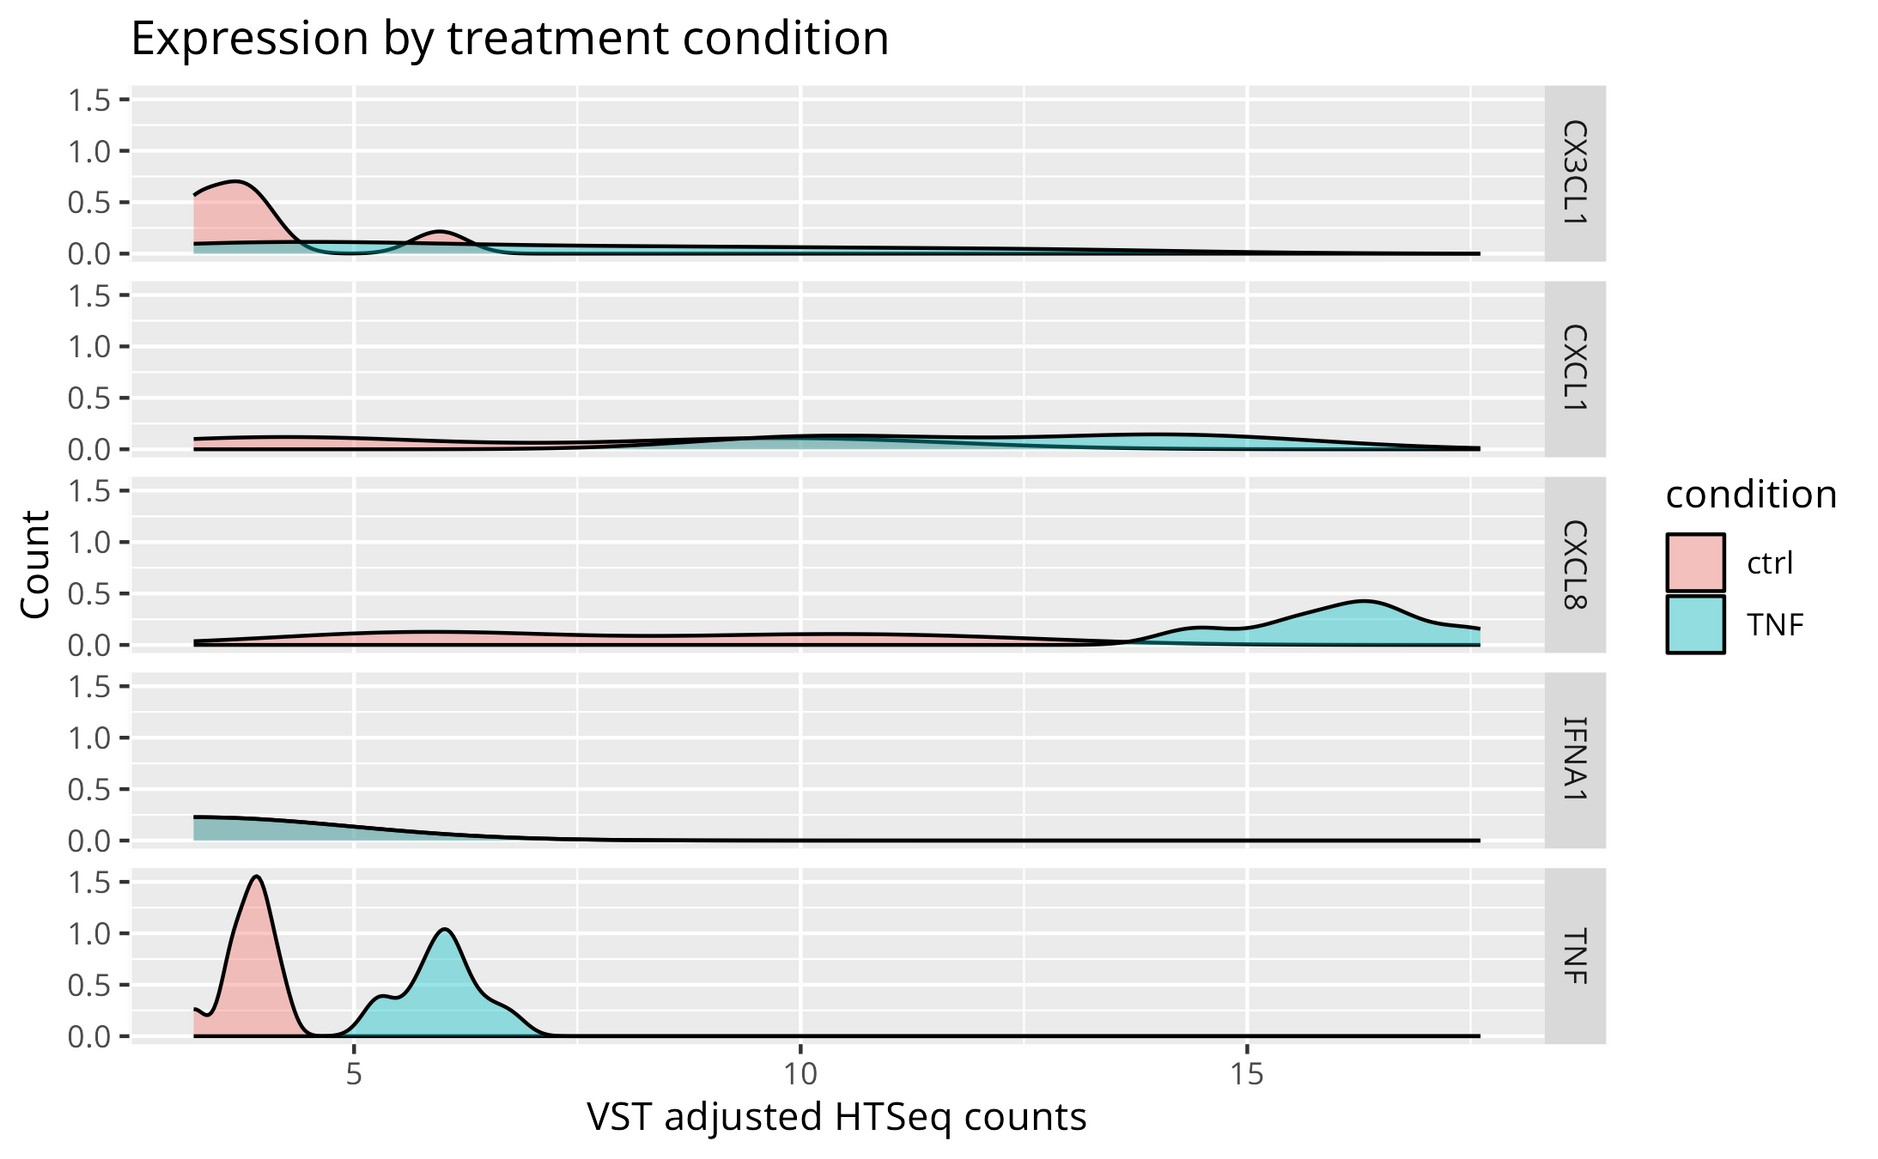
\includegraphics[width=0.7\linewidth]{chapters/images/ecpc-018.png}
\caption{Density plots of VST adjust HTSeq counts for several key indicator genes, visualised via breakdowns across multiple axes. Across all axes the distribution is generally not normal but often bimodal or without a defined distribution pattern.}\label{figure:sup1}
\end{figure}

\begin{figure}[bt!]
\centering
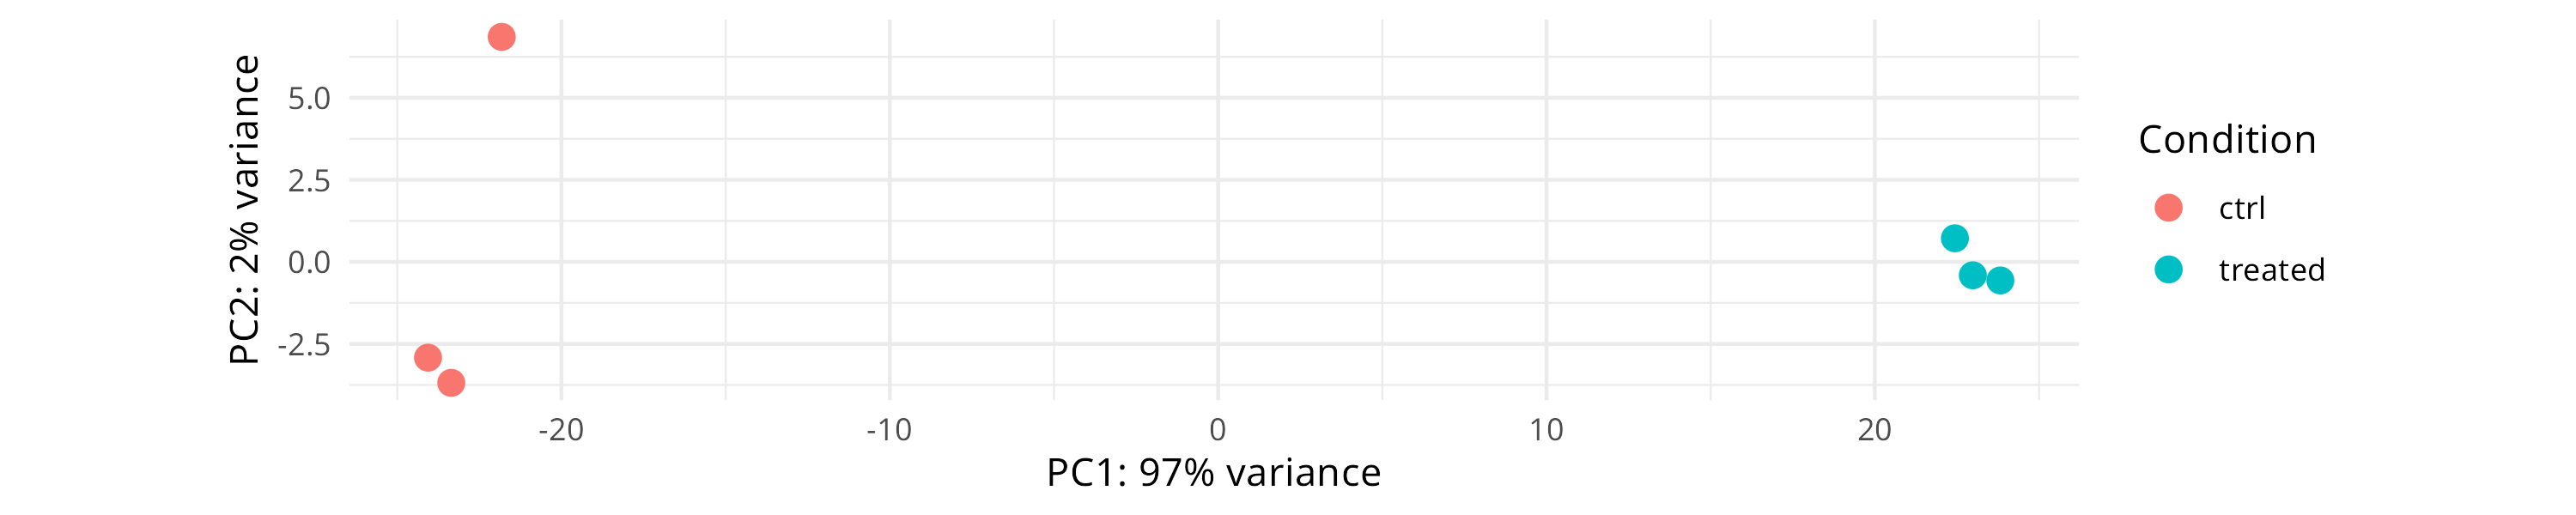
\includegraphics[width=\linewidth]{chapters/images/ecpc/7-pca.png}
\caption{Essentially all variance observed (97\%) is due to the treatment axis.}\label{figure:sup2}
\end{figure}

\footnotesize
\bibliographystyle{hexy.bst}
\bibliography{references}
\normalsize
